

\section{Tables}
\label{sec:tables}

\begin{table}[htbp]
    \centering
    \begin{tabular}{c| c}
        
        Year & State \\
        \hline \hline
        2005 & Texas \\
        2006 & Arkansas \\
        2006 & Oklahoma \\
        2008 & Alabama \\
        2008 & Louisiana \\
        2008 & Pennsylvania \\
        2008 & West Virginia \\
    \end{tabular}
    \caption{Shale Gas Extraction Beginnings by State}
    \label{tab:shale-gas-extraction}
\end{table}


\begin{table}[ht]
\centering
\tiny
\begin{tabular}{l|l||c|c|ccc|ccc}
  \hline 
 & Age  & Observations & Weighted Population & \multicolumn{3}{c|}{Personal Income} & \multicolumn{3}{c}{Family Income} \\ 
 &  & & & Mean & Std. Dev. & Count & Mean & Std. Dev. & Count\\ 
  \hline 
   \multirow{4}{*}{Non-shale} & [5, 10] & 1,308,465.00 & 170,364,982.00 & NaN & -0.00 & 0.00 & 72,838.58 & 75,229.40 & 1,298,525.00 \\ 
   & [16, 18] & 716,276.00 & 89,493,317.00 & 2,152.02 & 5,346.15 & 716,139.00 & 76,209.93 & 75,288.26 & 684,920.00 \\ 
   & [18, 24] & 1,396,758.00 & 201,384,880.00 & 10,645.98 & 13,378.58 & 1,396,368.00 & 59,542.08 & 63,236.34 & 1,287,939.00 \\ 
   & total & 17,029,516.00 & 2,116,225,634.00 & 32,089.57 & 45,426.91 & 13,756,814.00 & 71,707.67 & 72,064.18 & 16,680,293.00 \\ 
   \multirow{4}{*}{Shale} & [5, 10] & 301,477.00 & 40,178,779.00 & NaN & -0.00 & 0.00 & 62,547.86 & 64,017.72 & 299,038.00 \\ 
   & [16, 18] & 162,607.00 & 20,788,610.00 & 2,107.18 & 5,266.69 & 162,587.00 & 67,489.58 & 66,903.25 & 155,650.00 \\ 
   & [18, 24] & 315,031.00 & 47,152,003.00 & 10,024.05 & 12,636.98 & 314,959.00 & 52,141.72 & 55,290.96 & 291,304.00 \\ 
   & total & 3,794,579.00 & 478,463,294.00 & 28,501.66 & 40,124.54 & 3,043,685.00 & 63,292.86 & 62,940.60 & 3,709,749.00 \\ 
   \hline \hline
   & Age & \multirow{10}{*}{} & \multirow{10}{*}{}& \multicolumn{3}{c|}{Education (Years)} & \multicolumn{3}{c}{College Enrollment} \\ 
  & &  & & Mean & Std. Dev. & Count  & Mean & Std. Dev. & Count  \\ 
  \hline
   \multirow{4}{*}{Non-shale} & [5, 10] & &  & 0.63 & 1.31 & 1,308,465.00 & 0.00 & 0.00 & 1,308,465.00 \\ 
   & [16, 18] & &  & 10.60 & 1.32 & 716,276.00 & 0.23 & 0.42 & 716,276.00 \\ 
   & [18, 24] &  &  & 12.37 & 2.02 & 1,396,758.00 & 0.82 & 0.39 & 1,396,758.00 \\ 
   & total &  & & 11.14 & 5.28 & 16,429,863.00 & 0.64 & 0.48 & 17,029,516.00 \\ 
   \multirow{4}{*}{Shale}& [5, 10] &  &  & 0.60 & 1.25 & 301,477.00 & 0.00 & 0.00 & 301,477.00 \\ 
   & [16, 18] &  &  & 10.48 & 1.40 & 162,607.00 & 0.21 & 0.41 & 162,607.00 \\ 
   & [18, 24] &  &  & 12.22 & 2.00 & 315,031.00 & 0.80 & 0.40 & 315,031.00 \\ 
   & total &  &  & 10.74 & 5.21 & 3,656,064.00 & 0.61 & 0.49 & 3,794,579.00 \\ 
   \hline
\end{tabular}
\caption{Summary Statistics} 
\label{tab:sum_stat}
\end{table}


\newpage
\section{Figures}


% \begin{figure}[htbp]
%     \centering
%     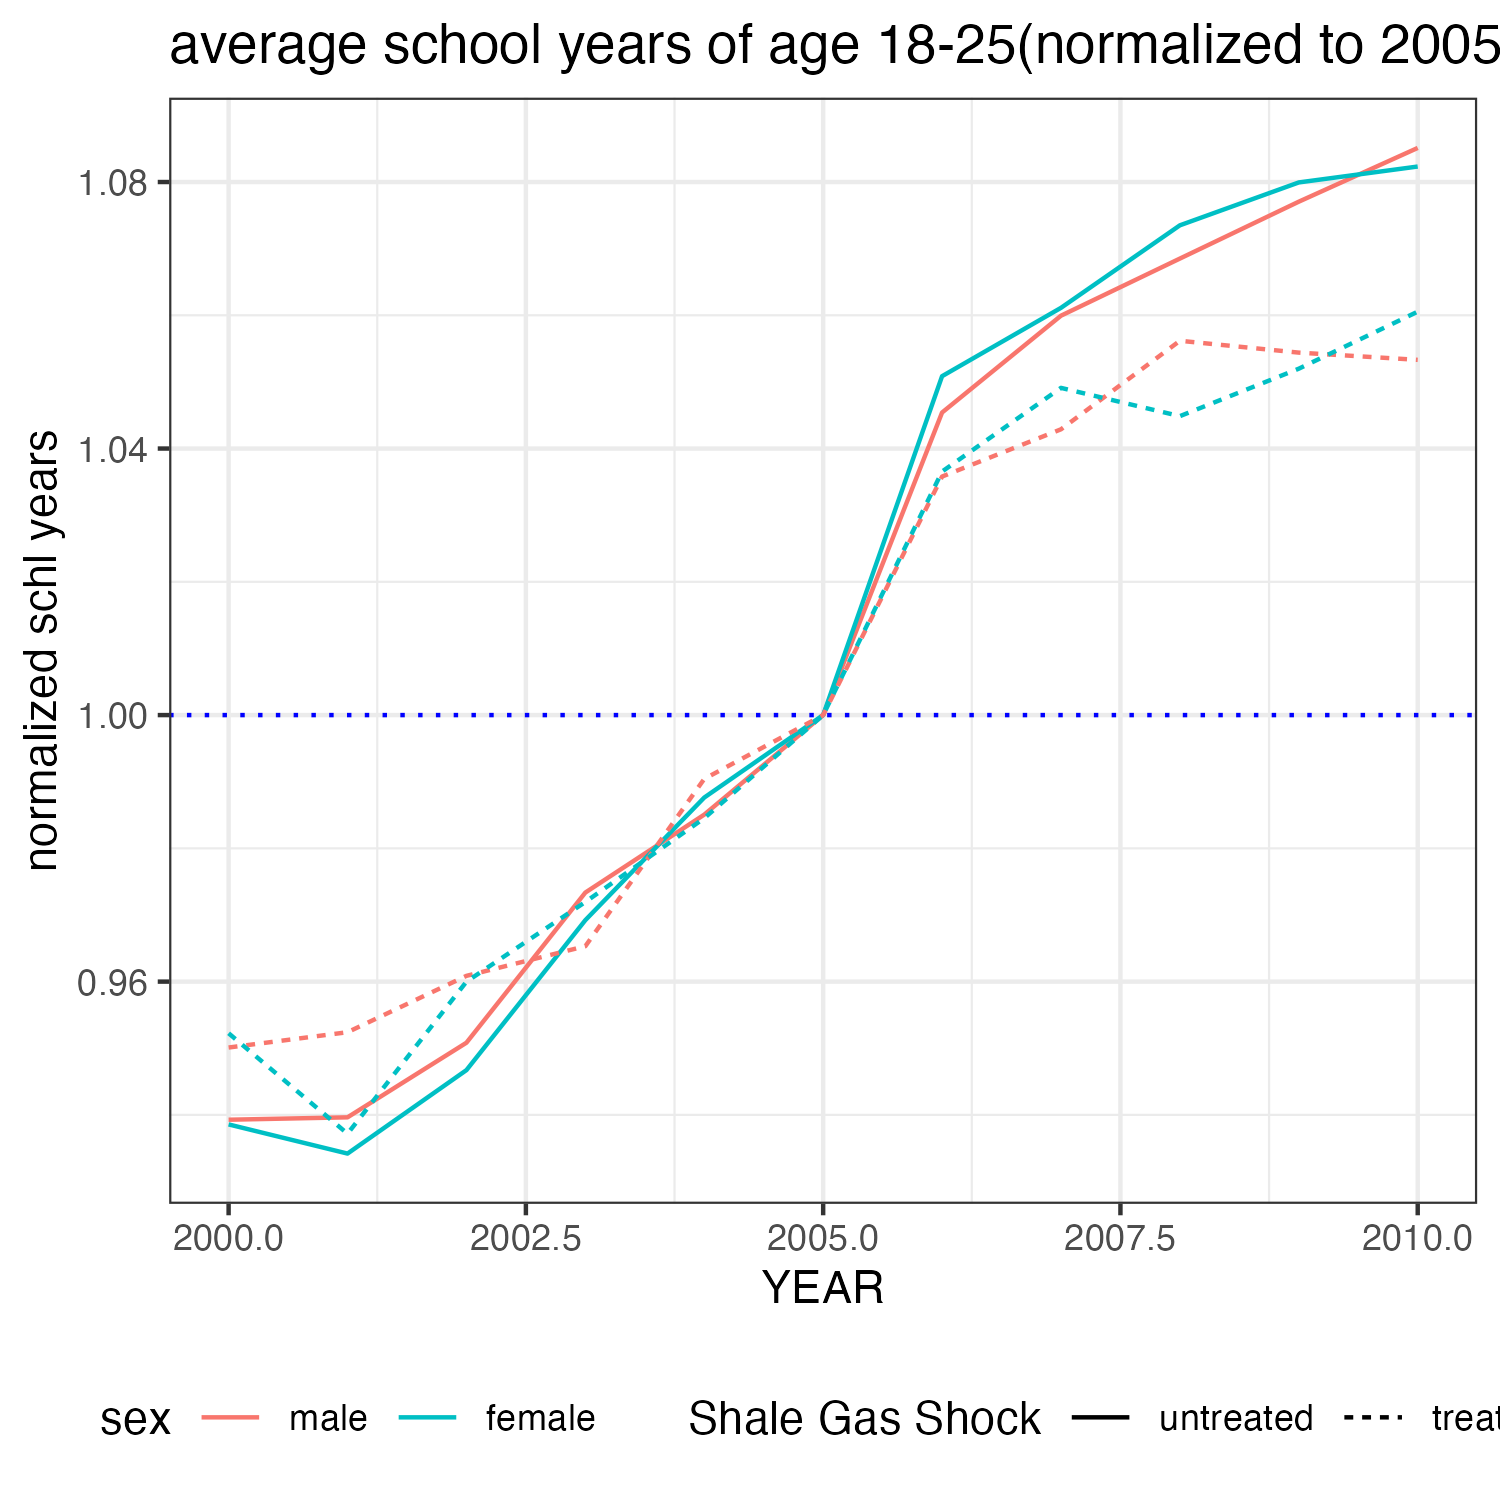
\includegraphics[width=0.4\textwidth]{figures/did-base/fig1.png}
%     \caption{Impact of Shale Gas Boom on Average Schooling Years}
%     \label{fig:did-base-fig1}
%     \begin{minipage}{10cm}
%     \scriptsize
%     Notes:
%     \end{minipage}
% \end{figure}

\begin{figure}[htbp]
    \centering
    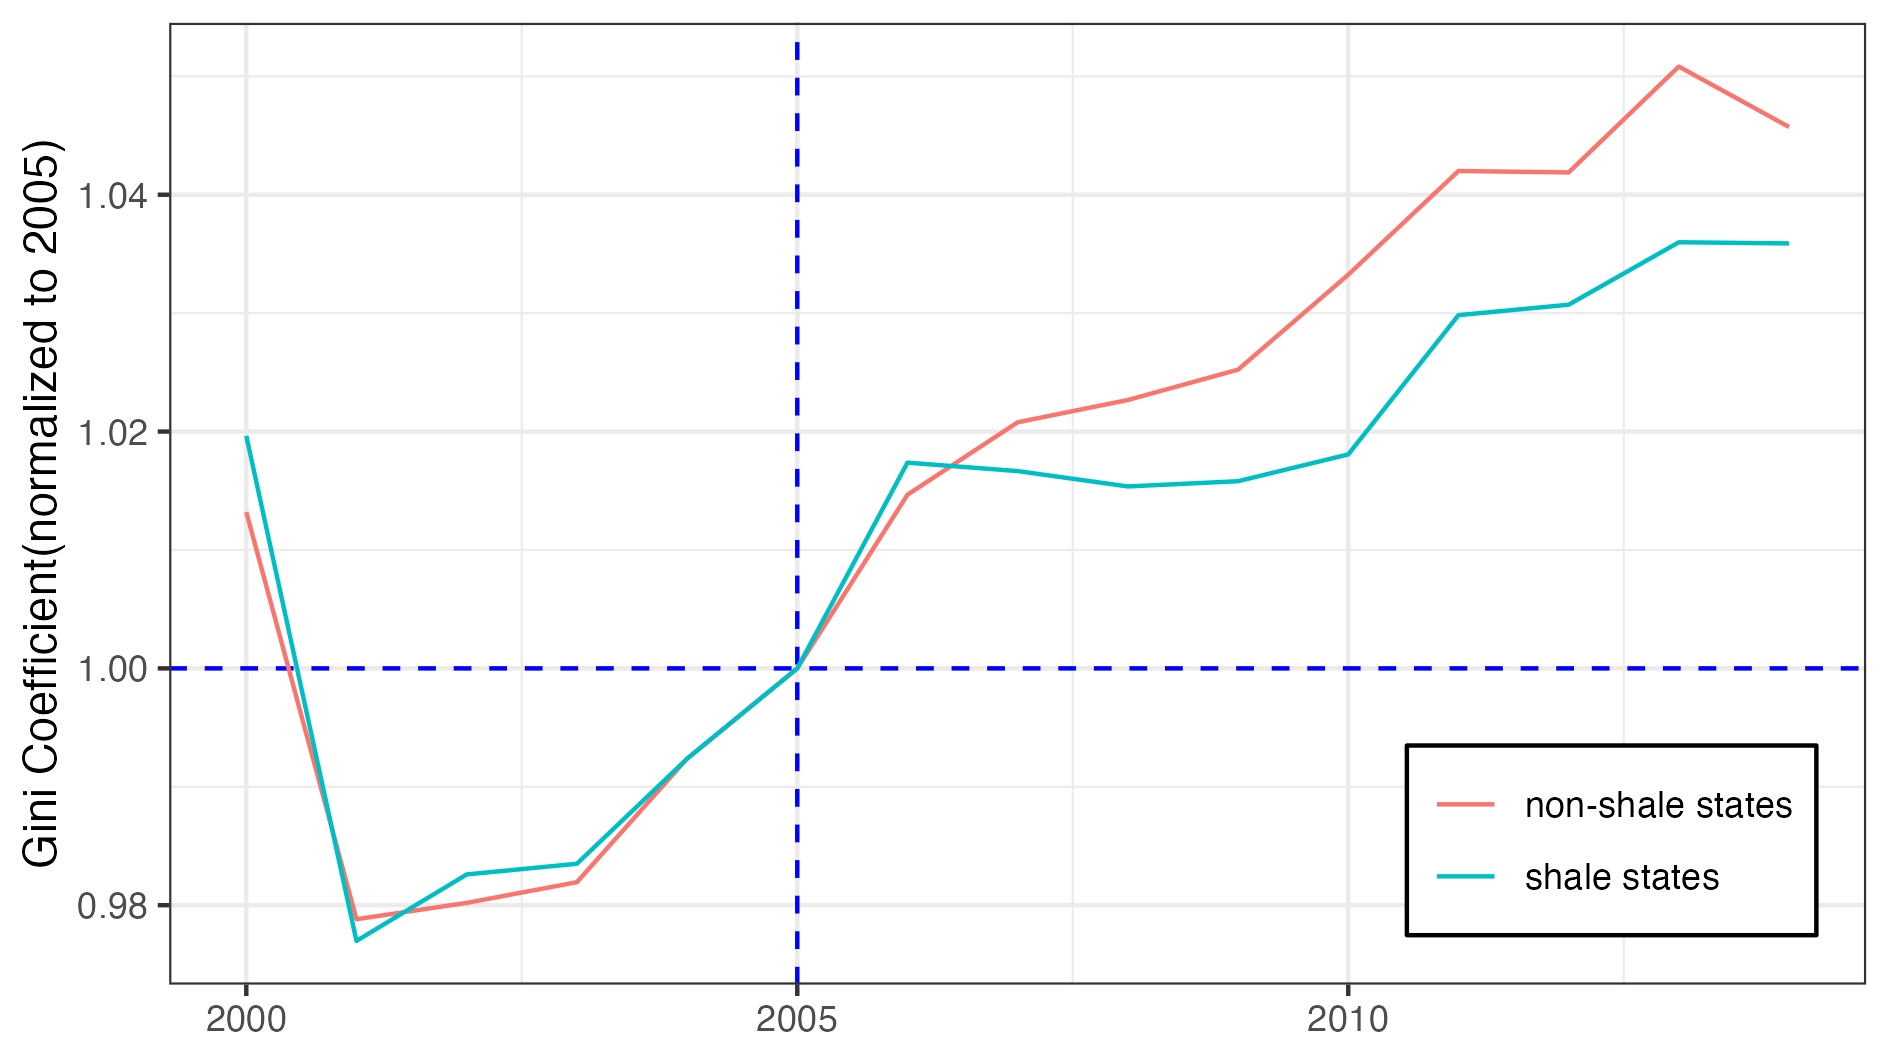
\includegraphics[width=0.7\textwidth]{figures/gini.png}
    \captionsetup{width=0.7\textwidth}
    \caption{Gini Coefficient by Treatment Status}
    \label{fig:gini}
    \begin{minipage}{0.7\textwidth}
    \scriptsize
    Notes: The Gini coefficient is computed within the ACS yearly data for each state, based on individual yearly income. 
    Individuals without income infomrmation or with negative net income are excluded from the calculation, and the Gini coefficient in the figure 
    is normalized to the 2005 level of each respective group.
    \end{minipage}
\end{figure}

\begin{figure}[htbp]
    \centering
    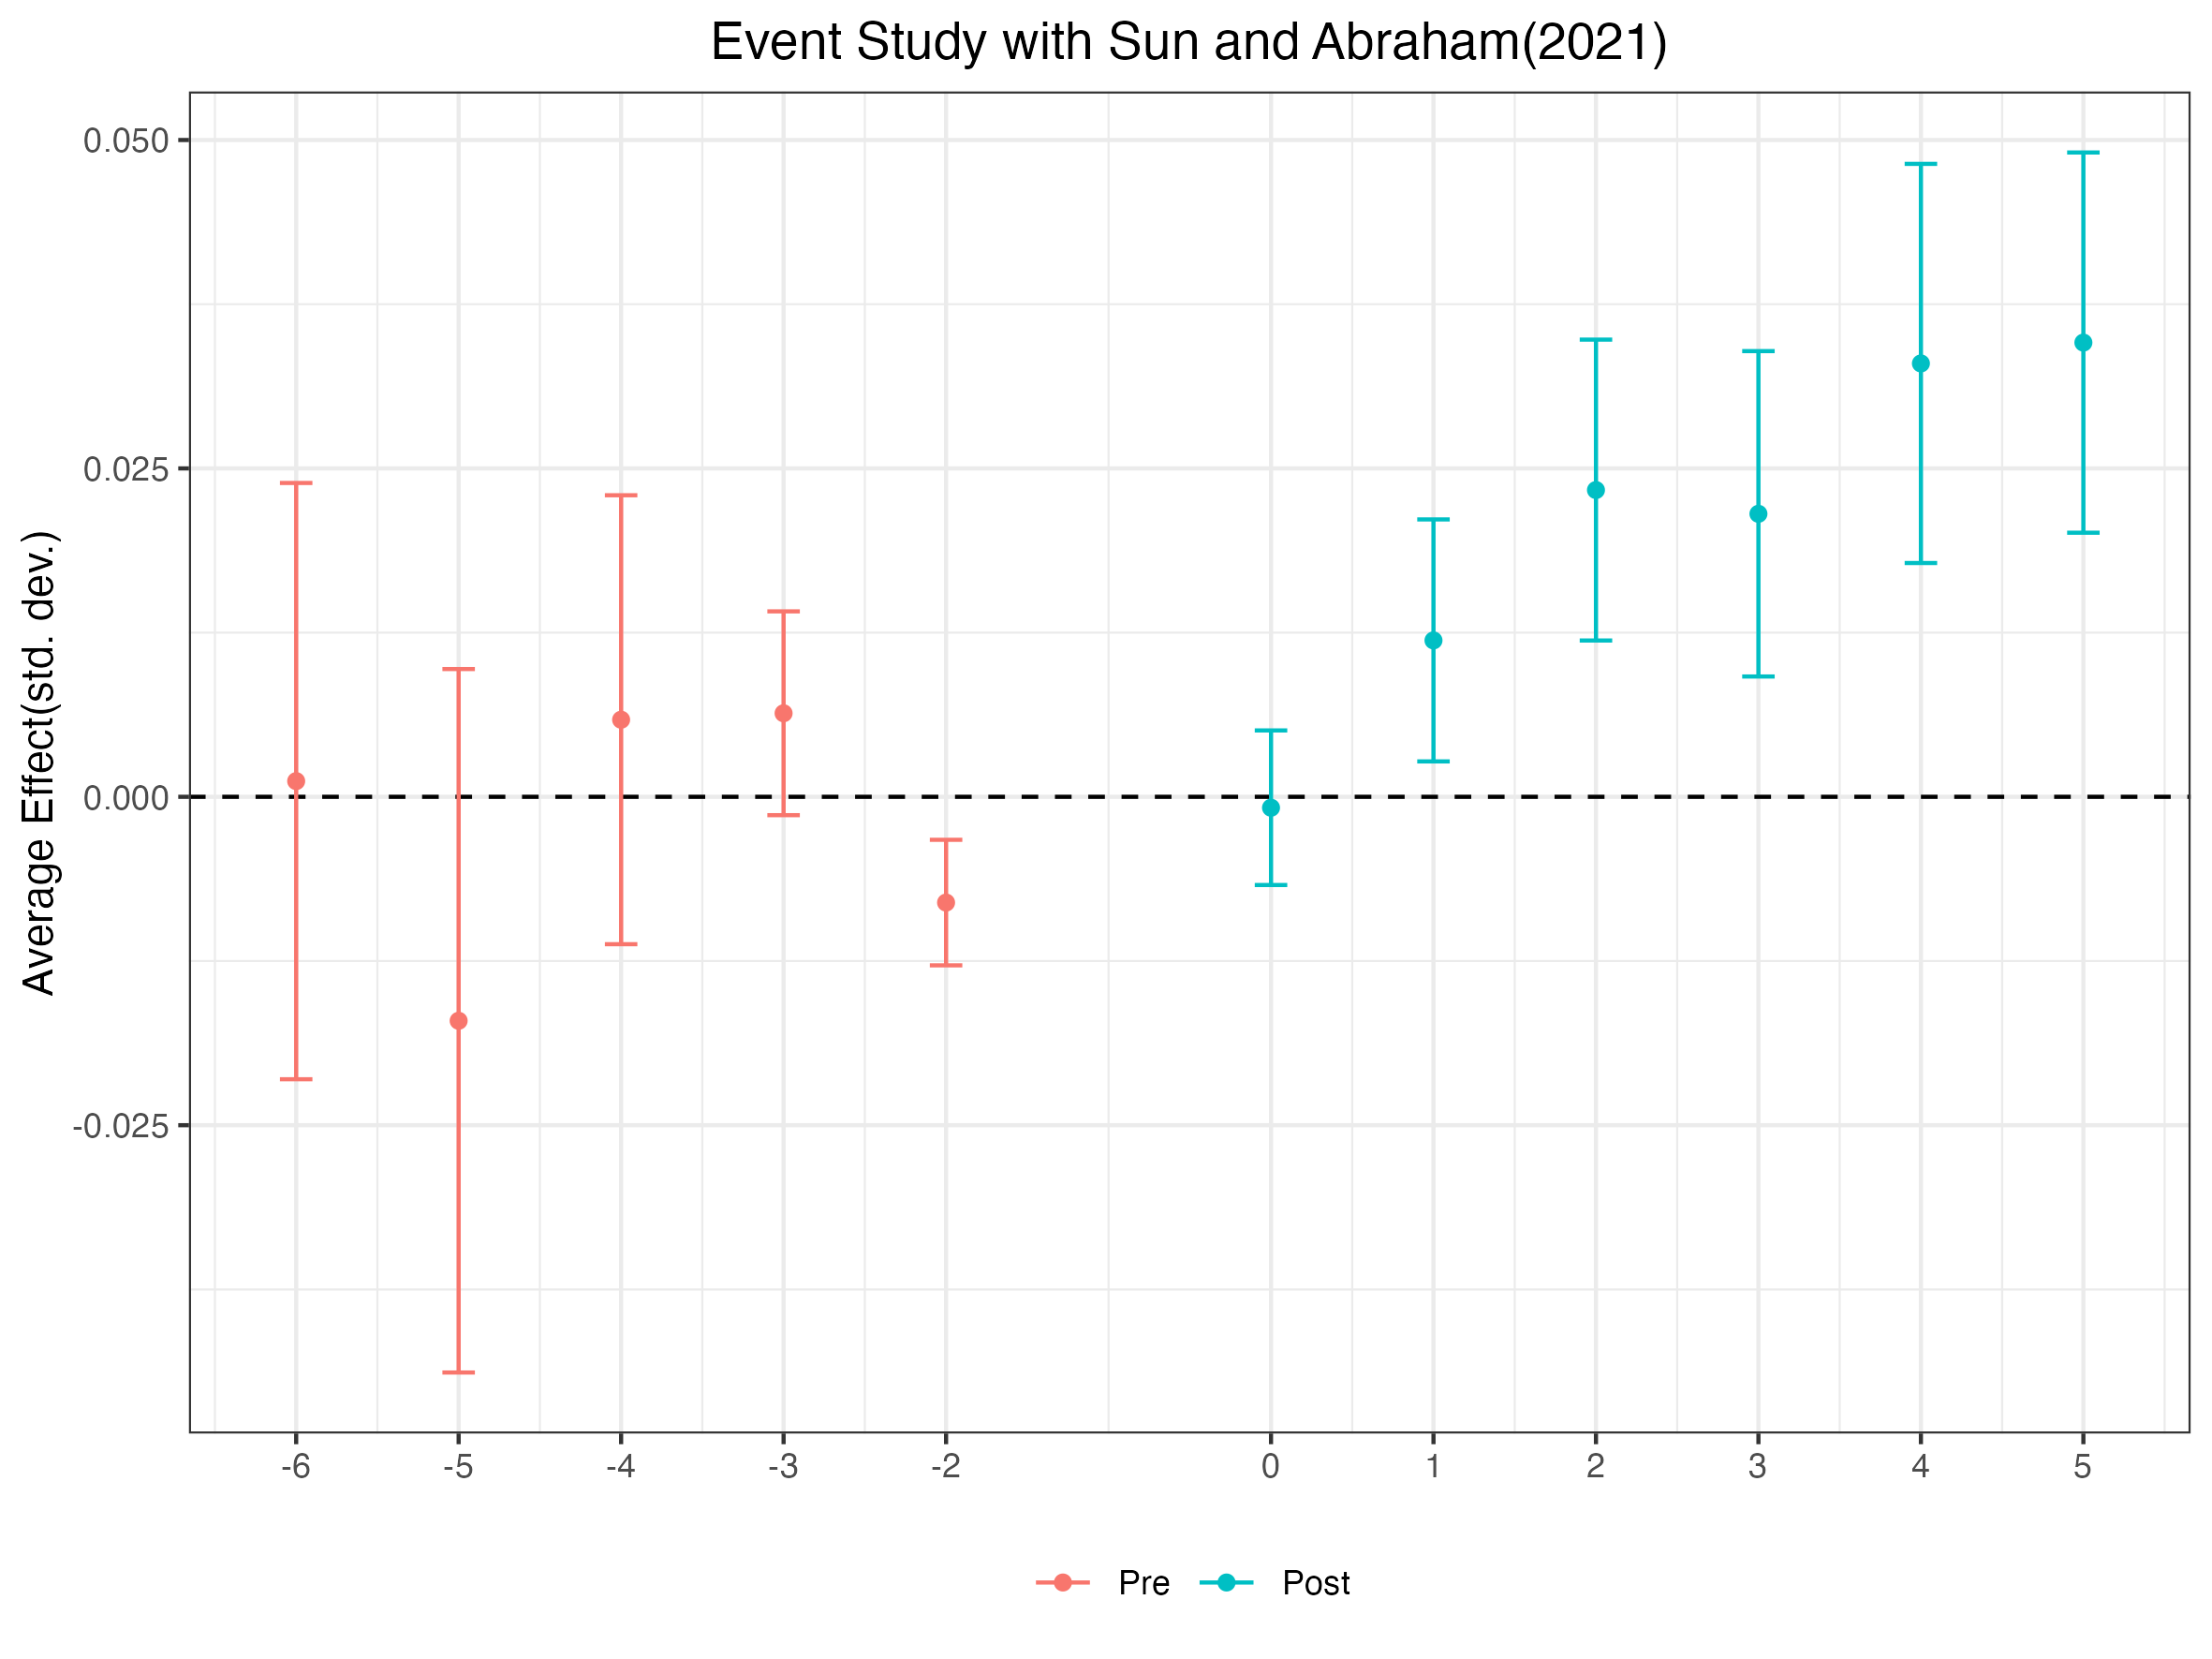
\includegraphics[width=0.7\textwidth, height=8.5cm]{figures/did-base/sadid(logFTOTINC).png}
    \captionsetup{width=0.7\textwidth}
    \caption{Event Study: Overall Household Income}
    \label{fig:Overall Income}
    \begin{minipage}{0.7\textwidth}
    \scriptsize
    Notes: The figure shows the event study results of the household income based on SA-DiD. 
    The base period is set to the year before the shale boom started in each state.
    The point estimates can be interpreted as the percentage change in household income with respect to the treatment (i.e., the shale boom).
    Standard errors are clustered at the state level and the confidence intervals shown are 95\% confidence intervals.
    \end{minipage}
\end{figure}

\begin{figure}[htbp]
    \centering
    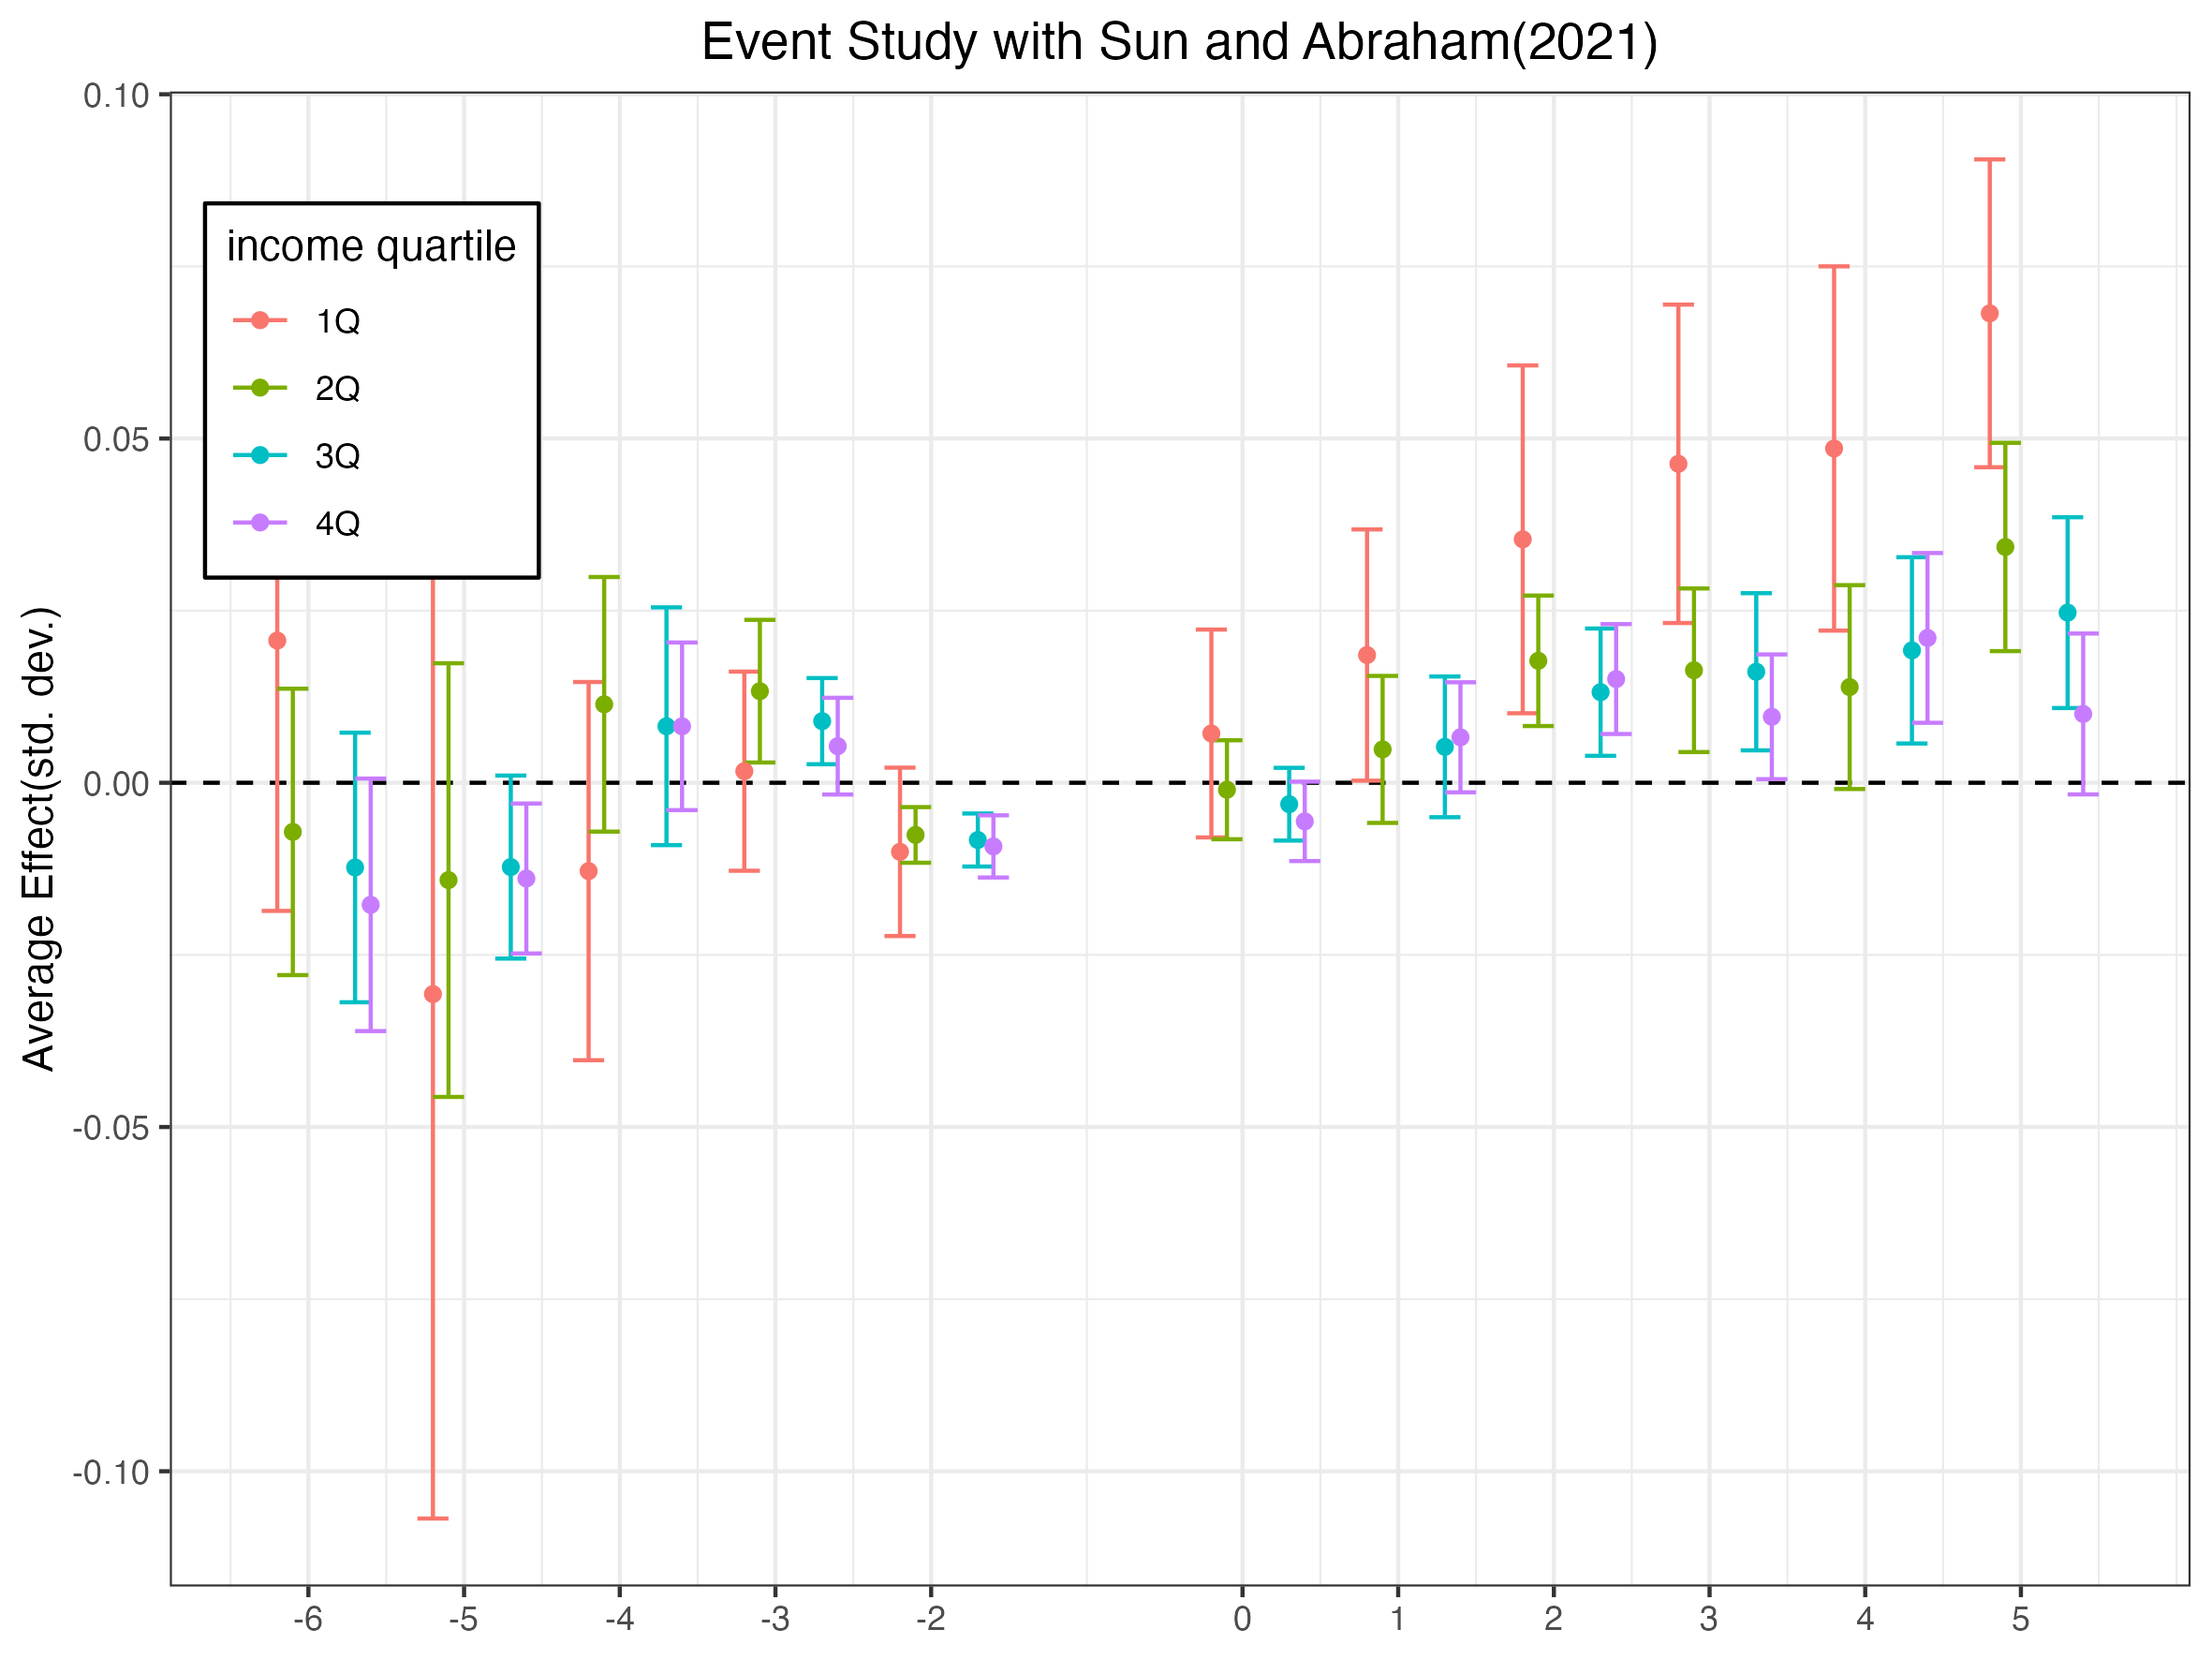
\includegraphics[width=0.7\textwidth]{figures/did-base/sadid(logFTOTINC - by income quartile).png}
    \captionsetup{width=0.7\textwidth}
    \caption{Event Study: Household Income by Quartile}
    \label{fig:Income by Quartile}
    \begin{minipage}{0.7\textwidth}
    \scriptsize
    Notes: The figure shows the event study results of the household income by income quartile based on SA-DiD. 
    The base period is set to the year before the shale boom started in each state.
    The point estimates can be interpreted as the percentage change in household income with respect to the treatment (i.e., the shale boom).
    Standard errors are clustered at the state level and the confidence intervals shown are 95\% confidence intervals.
    Also, note that the cutoffs for income quartiles are nation-level quartiles adjusted by the sampling weights and is fluctuant across years.
    \end{minipage}
\end{figure}

\begin{figure}[htbp]
    \centering
    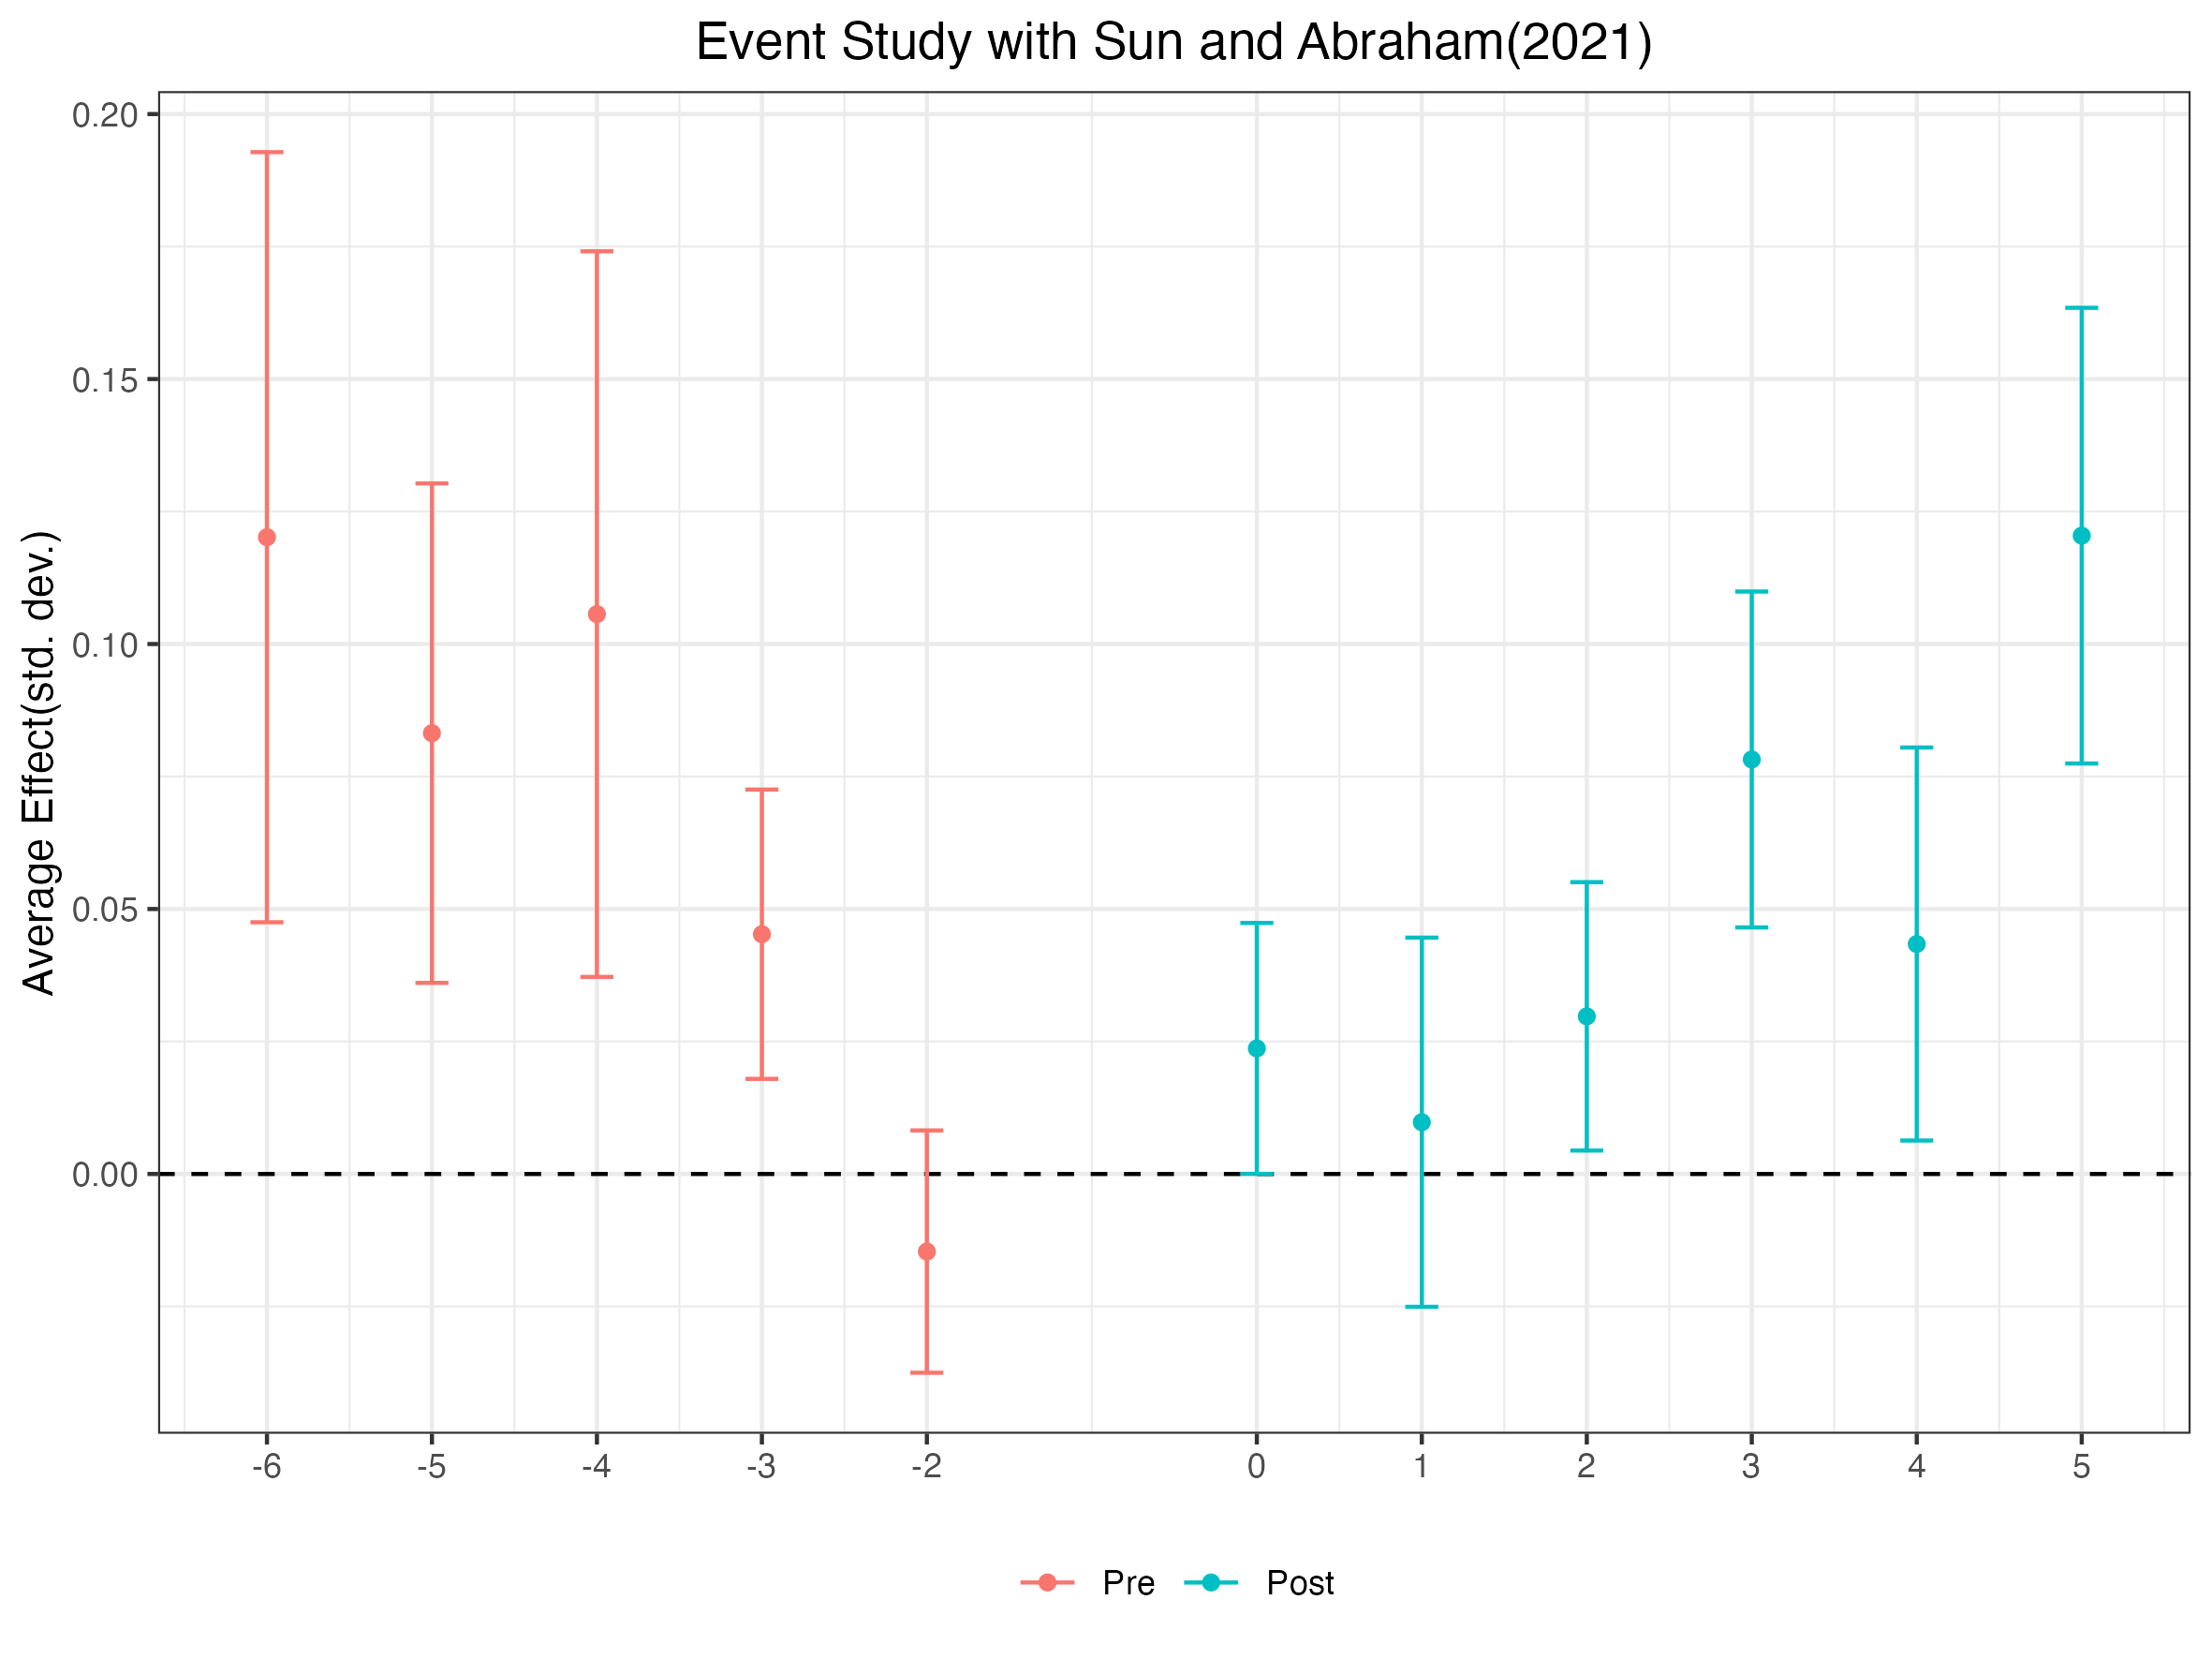
\includegraphics[width=0.7\textwidth, height=8.5cm]{figures/did-base/sadid(college enrollment).png}
    \captionsetup{width=0.7\textwidth}
    \caption{Event Study: Overall College Enrollment}
    \label{fig:college shares}
    \begin{minipage}{0.7\textwidth}
    \scriptsize
    Notes: The figure shows the event study results of the college enrollment among individuals between age 18 and 24 (inclusive) based on SA-DiD. 
    The base period is set to the year before the shale boom started in each state.
    The point estimates can be interpreted as the percentage point change in college enrollment status with respect to the treatment (i.e., the shale boom).
    Standard errors are clustered at the state level and the confidence intervals shown are 95\% confidence intervals.
    \end{minipage}
\end{figure}

\begin{figure}[htbp]
    \centering
    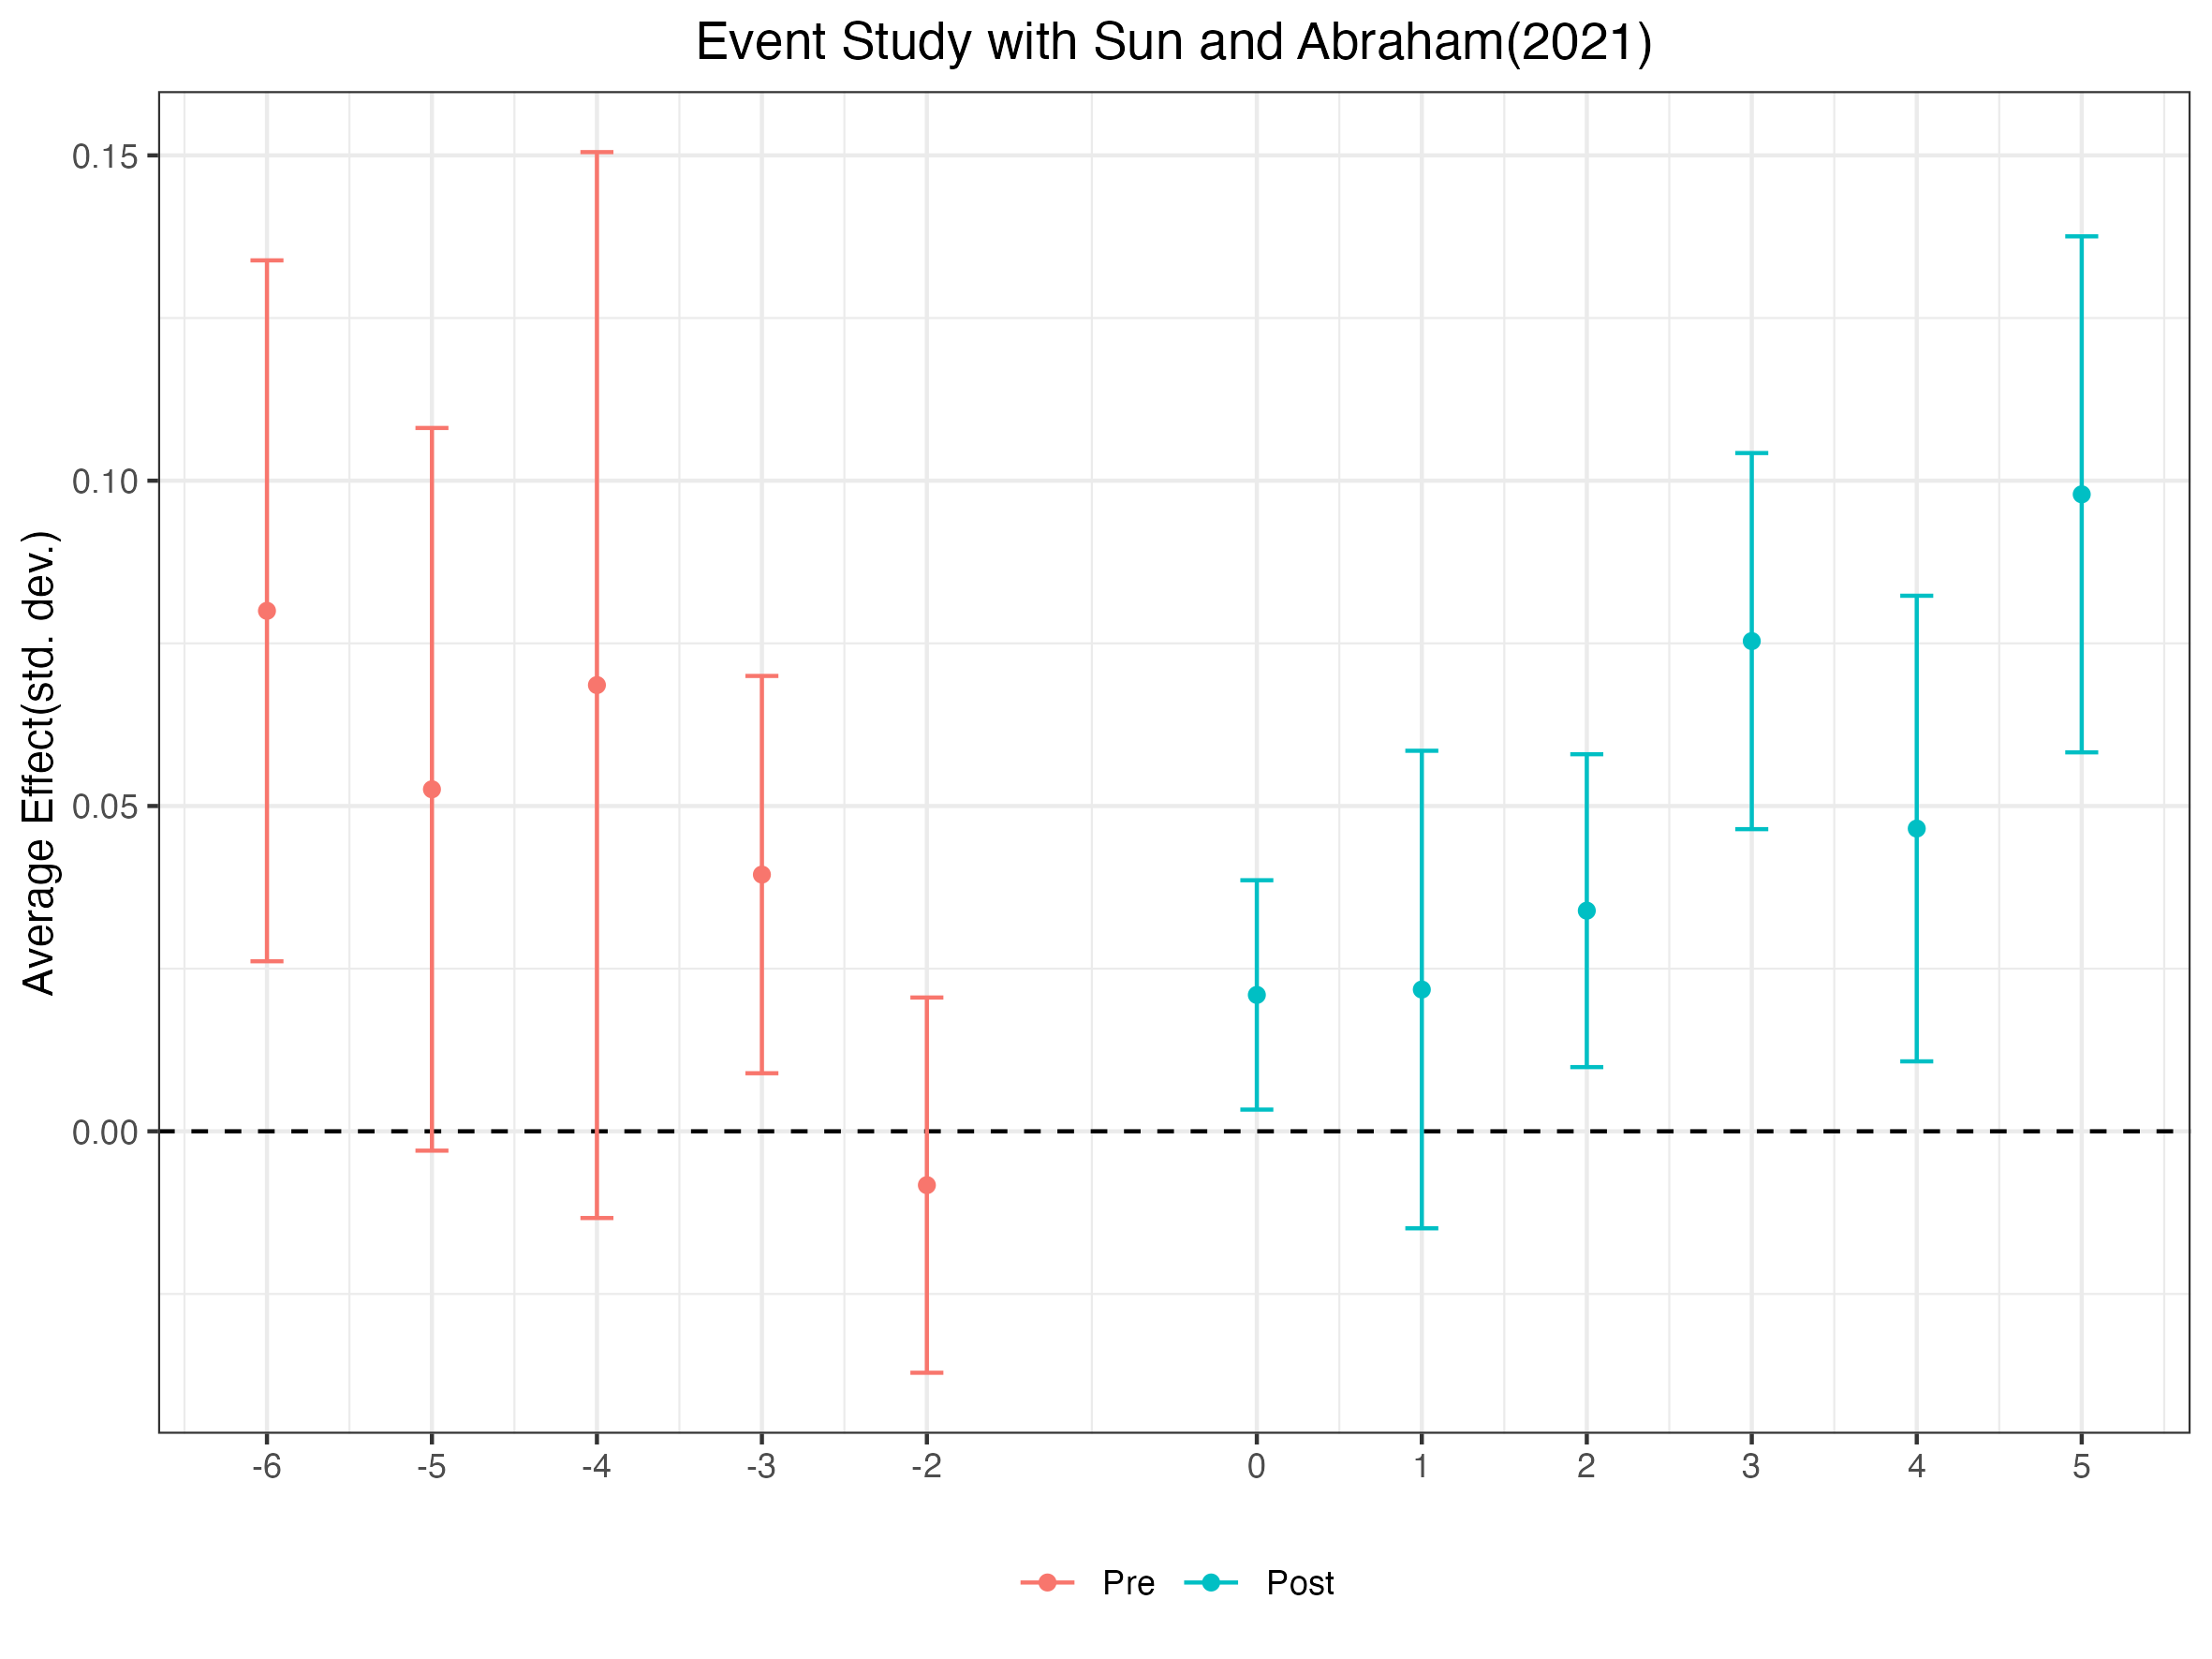
\includegraphics[width=0.7\textwidth, height=8.5cm]{figures/did-base/sadid(college enrollment - controls).png}
    \captionsetup{width=0.7\textwidth}
    \caption{Event Study: Overall College Enrollment (with Controls)}
    \label{fig:college shares-controls}
    \begin{minipage}{0.7\textwidth}
    \scriptsize
    Notes: The figure shows the event study results of the college enrollment among individuals between age 18 and 24 (inclusive) based on SA-DiD with covariates. 
    Covariates include sex, race, and household income of the individual.
    The base period is set to the year before the shale boom started in each state.
    The point estimates can be interpreted as the percentage point change in college enrollment status with respect to the treatment (i.e., the shale boom).
    Standard errors are clustered at the state level and the confidence intervals shown are 95\% confidence intervals.
    \end{minipage}
\end{figure}

\begin{figure}[htbp]
    \centering
    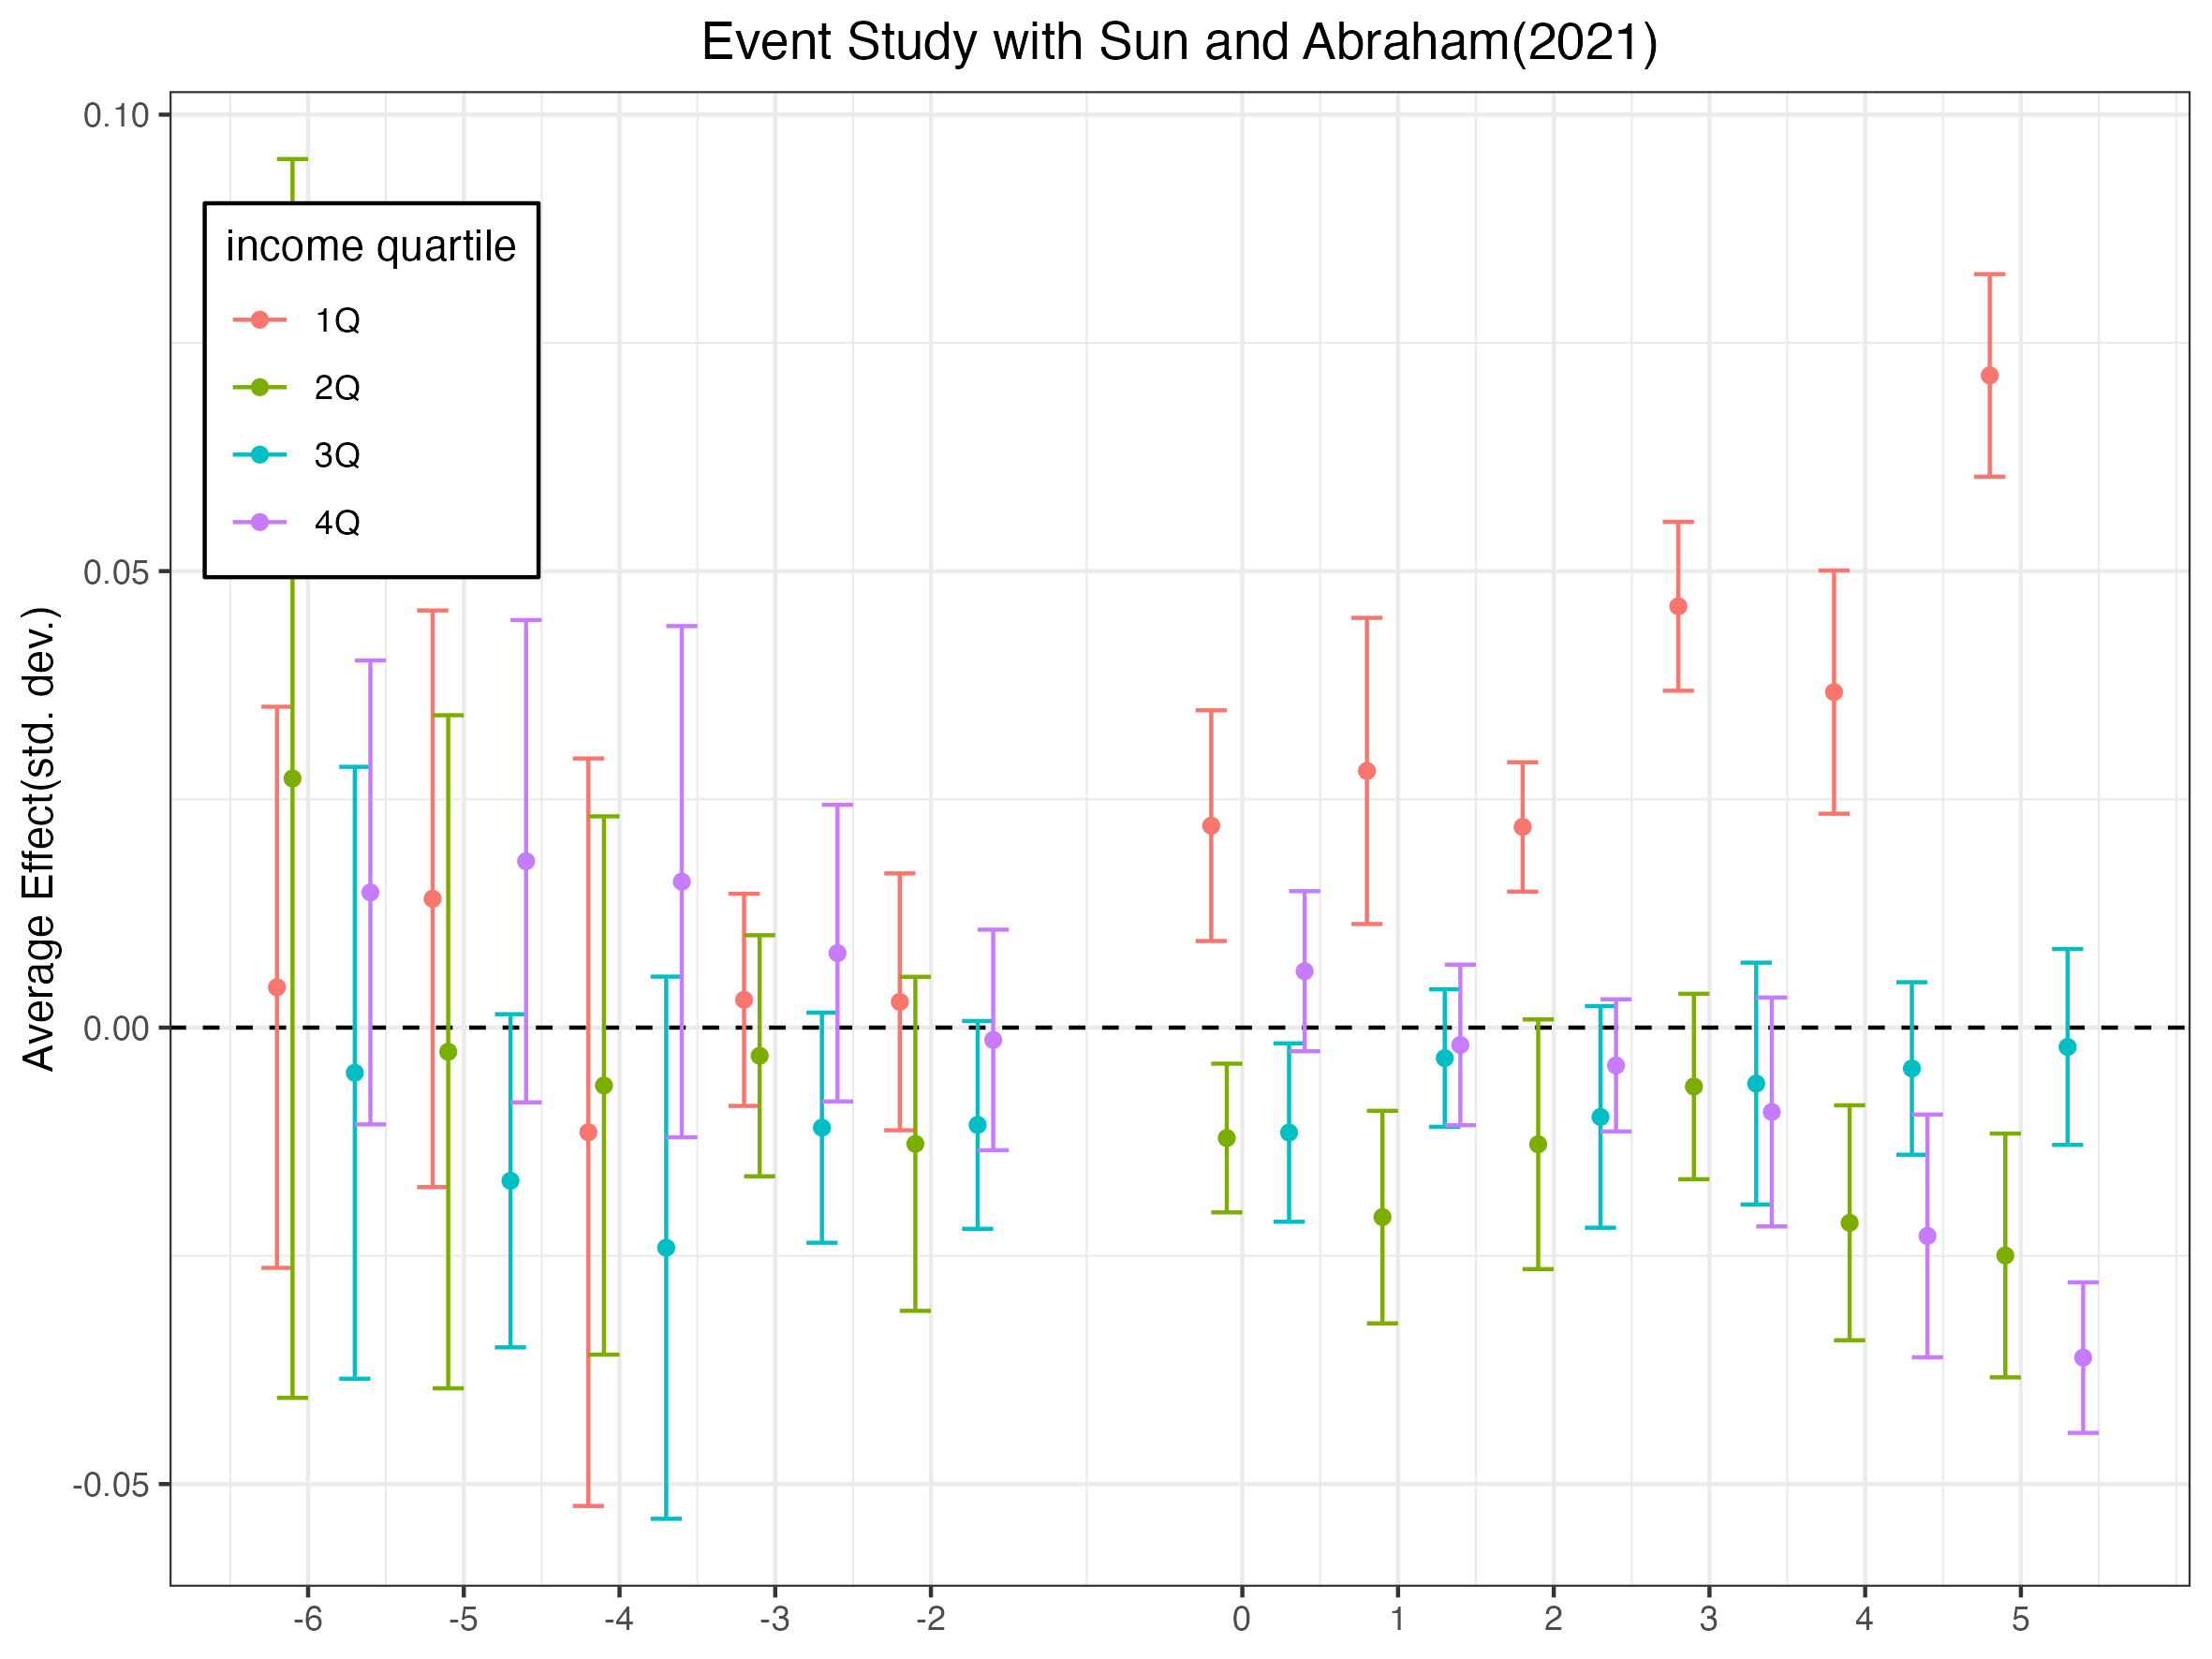
\includegraphics[width=0.7\textwidth]{figures/did-base/sadid(college share - by income quartile).png}
    \captionsetup{width=0.7\textwidth}
    \caption{Event Study: College Enrollment by Household Income Quartile}
    \label{fig:college enrollment}
    \begin{minipage}{0.7\textwidth}
    \scriptsize
    Notes: The figure shows the event study results of the college enrollment among individuals between age 18 and 24 (inclusive) by family income quartile based on SA-DiD. 
    The base period is set to the year before the shale boom started in each state.
    The point estimates can be interpreted as the percentage point change in college enrollment status with respect to the treatment (i.e., the shale boom).
    Standard errors are clustered at the state level and the confidence intervals shown are 95\% confidence intervals.
    Also, note that the cutoffs for income quartiles are nation-level quartiles adjusted by the sampling weights and is fluctuant across years.
    \end{minipage}
\end{figure}

\begin{figure}[htbp]
    \centering
    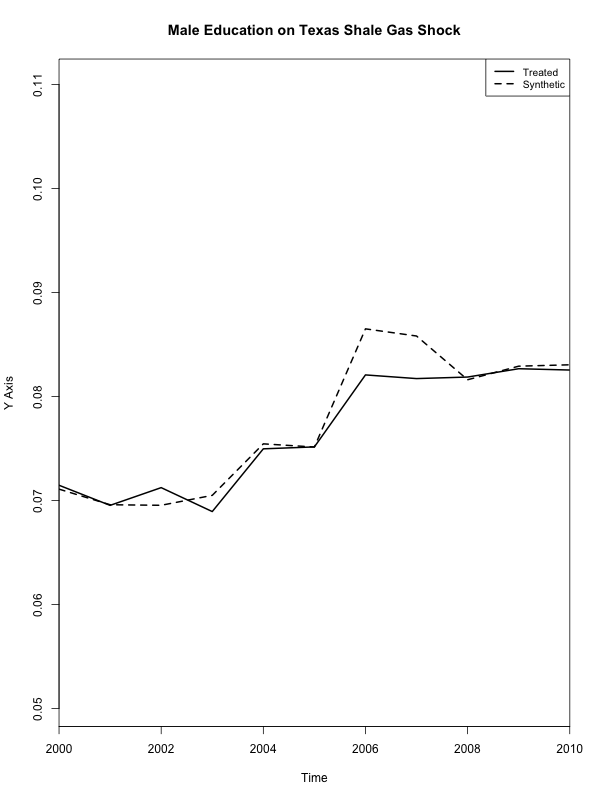
\includegraphics[width=0.7\textwidth]{figures/scm/fig3_v4.png}
    \captionsetup{width=0.7\textwidth}
    \caption{SCM Male Education}
    \label{fig:SCM male}
    \begin{minipage}{0.7\textwidth}
    \scriptsize
    Notes: The figure shows the synthetic control estimates of the college enrollment shares among
    males between age 18 and 24 (inclusive) in Texas, where the solid line represents Texas (the treated unit), and the dashed line corresponds to the synthetic control group.
    The weights for the synthetic control group are based on race composition, minor ratio (i.e., the ratio of individuals aged 0-17 to the total population), and population size
    in the pre-treatment period, which is defined as 2000 to 2005,
    inclusively.
    \end{minipage}
\end{figure}

\begin{figure}[htbp]
    \centering
    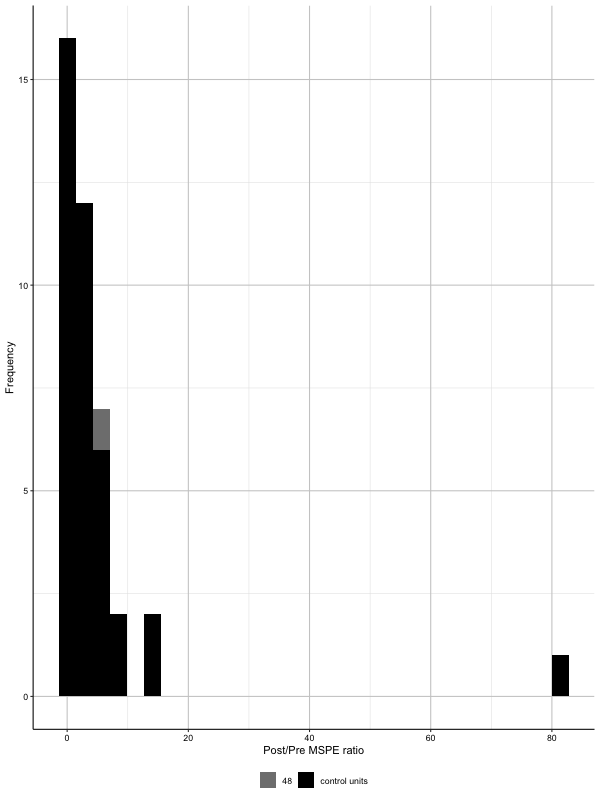
\includegraphics[width=0.7\textwidth]{figures/scm/fig3-mspe_v4.png}
    \captionsetup{width=0.7\textwidth}
    \caption{SCM Male Education MSPE}
    \label{fig:SCM male MSPE}
    \begin{minipage}{0.7\textwidth}
    \scriptsize
    Notes: The figure shows the post-treatment to pre-treatment mean squared prediction error (MSPE) ratio.
    The x-axis represents the MSPE ratio, and the y-axis represents the  frequency of the MSPE ratio.
    In the figure, the grey bar represents the MSPE ratio of Texas, and the black bars are MSPE ratios from having other states as placebo treated units.
    One can readily notice that the MSPE ratio of Texas is located at the left side of the distribution,
    implying that the actual post-treatment outcomes are predicted well by the synthetic control group;
    thus, the difference in college enrollment shares between Texas and its synthetic counterpart is not 
    unusually large relative to the placebo units whose MSPE ratios are shown in the same plot.
    \end{minipage}
\end{figure}

\begin{figure}[htbp]
    \centering
    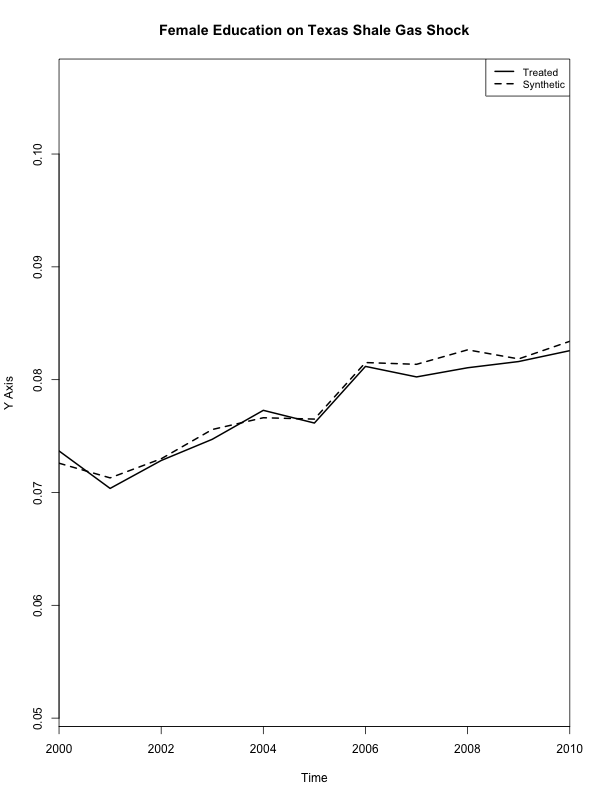
\includegraphics[width=0.7\textwidth]{figures/scm/fig4_v4.png}
    \captionsetup{width=0.7\textwidth}
    \caption{SCM Female Education}
    \label{fig:SCM female}
    \begin{minipage}{0.7\textwidth}
    \scriptsize
    Notes: The figure shows the synthetic control estimates of the college enrollment shares among
    females between age 18 and 24 (inclusive) in Texas, where the solid line represents Texas (the treated unit), and the dashed line corresponds to the synthetic control group.
    The weights for the synthetic control group are based on race composition, minor ratio (i.e., the ratio of individuals aged 0-17 to the total population), and population size
    in the pre-treatment period, which is defined as 2000 to 2005,
    inclusively.
    \end{minipage}
\end{figure}

% \begin{figure}[htbp]
%     \centering
%     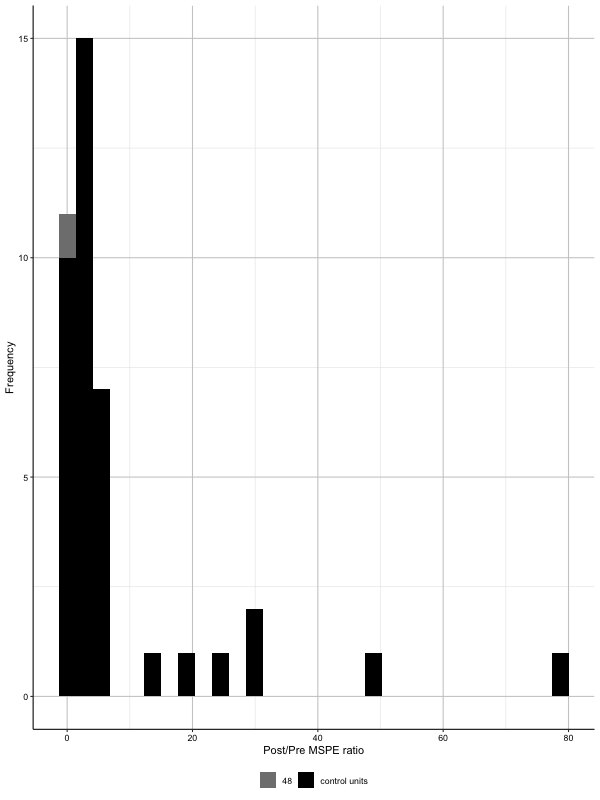
\includegraphics[width=0.7\textwidth]{figures/scm/fig4-mspe_v4.png}
%     \captionsetup{width=0.7\textwidth}
%     \caption{SCM Female Education MSPE}
%     \label{fig:SCM female MSPE}
%     \begin{minipage}{0.7\textwidth}
%     \scriptsize
%     Notes:
%     \end{minipage}
% \end{figure}


\begin{figure}[htbp]
    \centering
    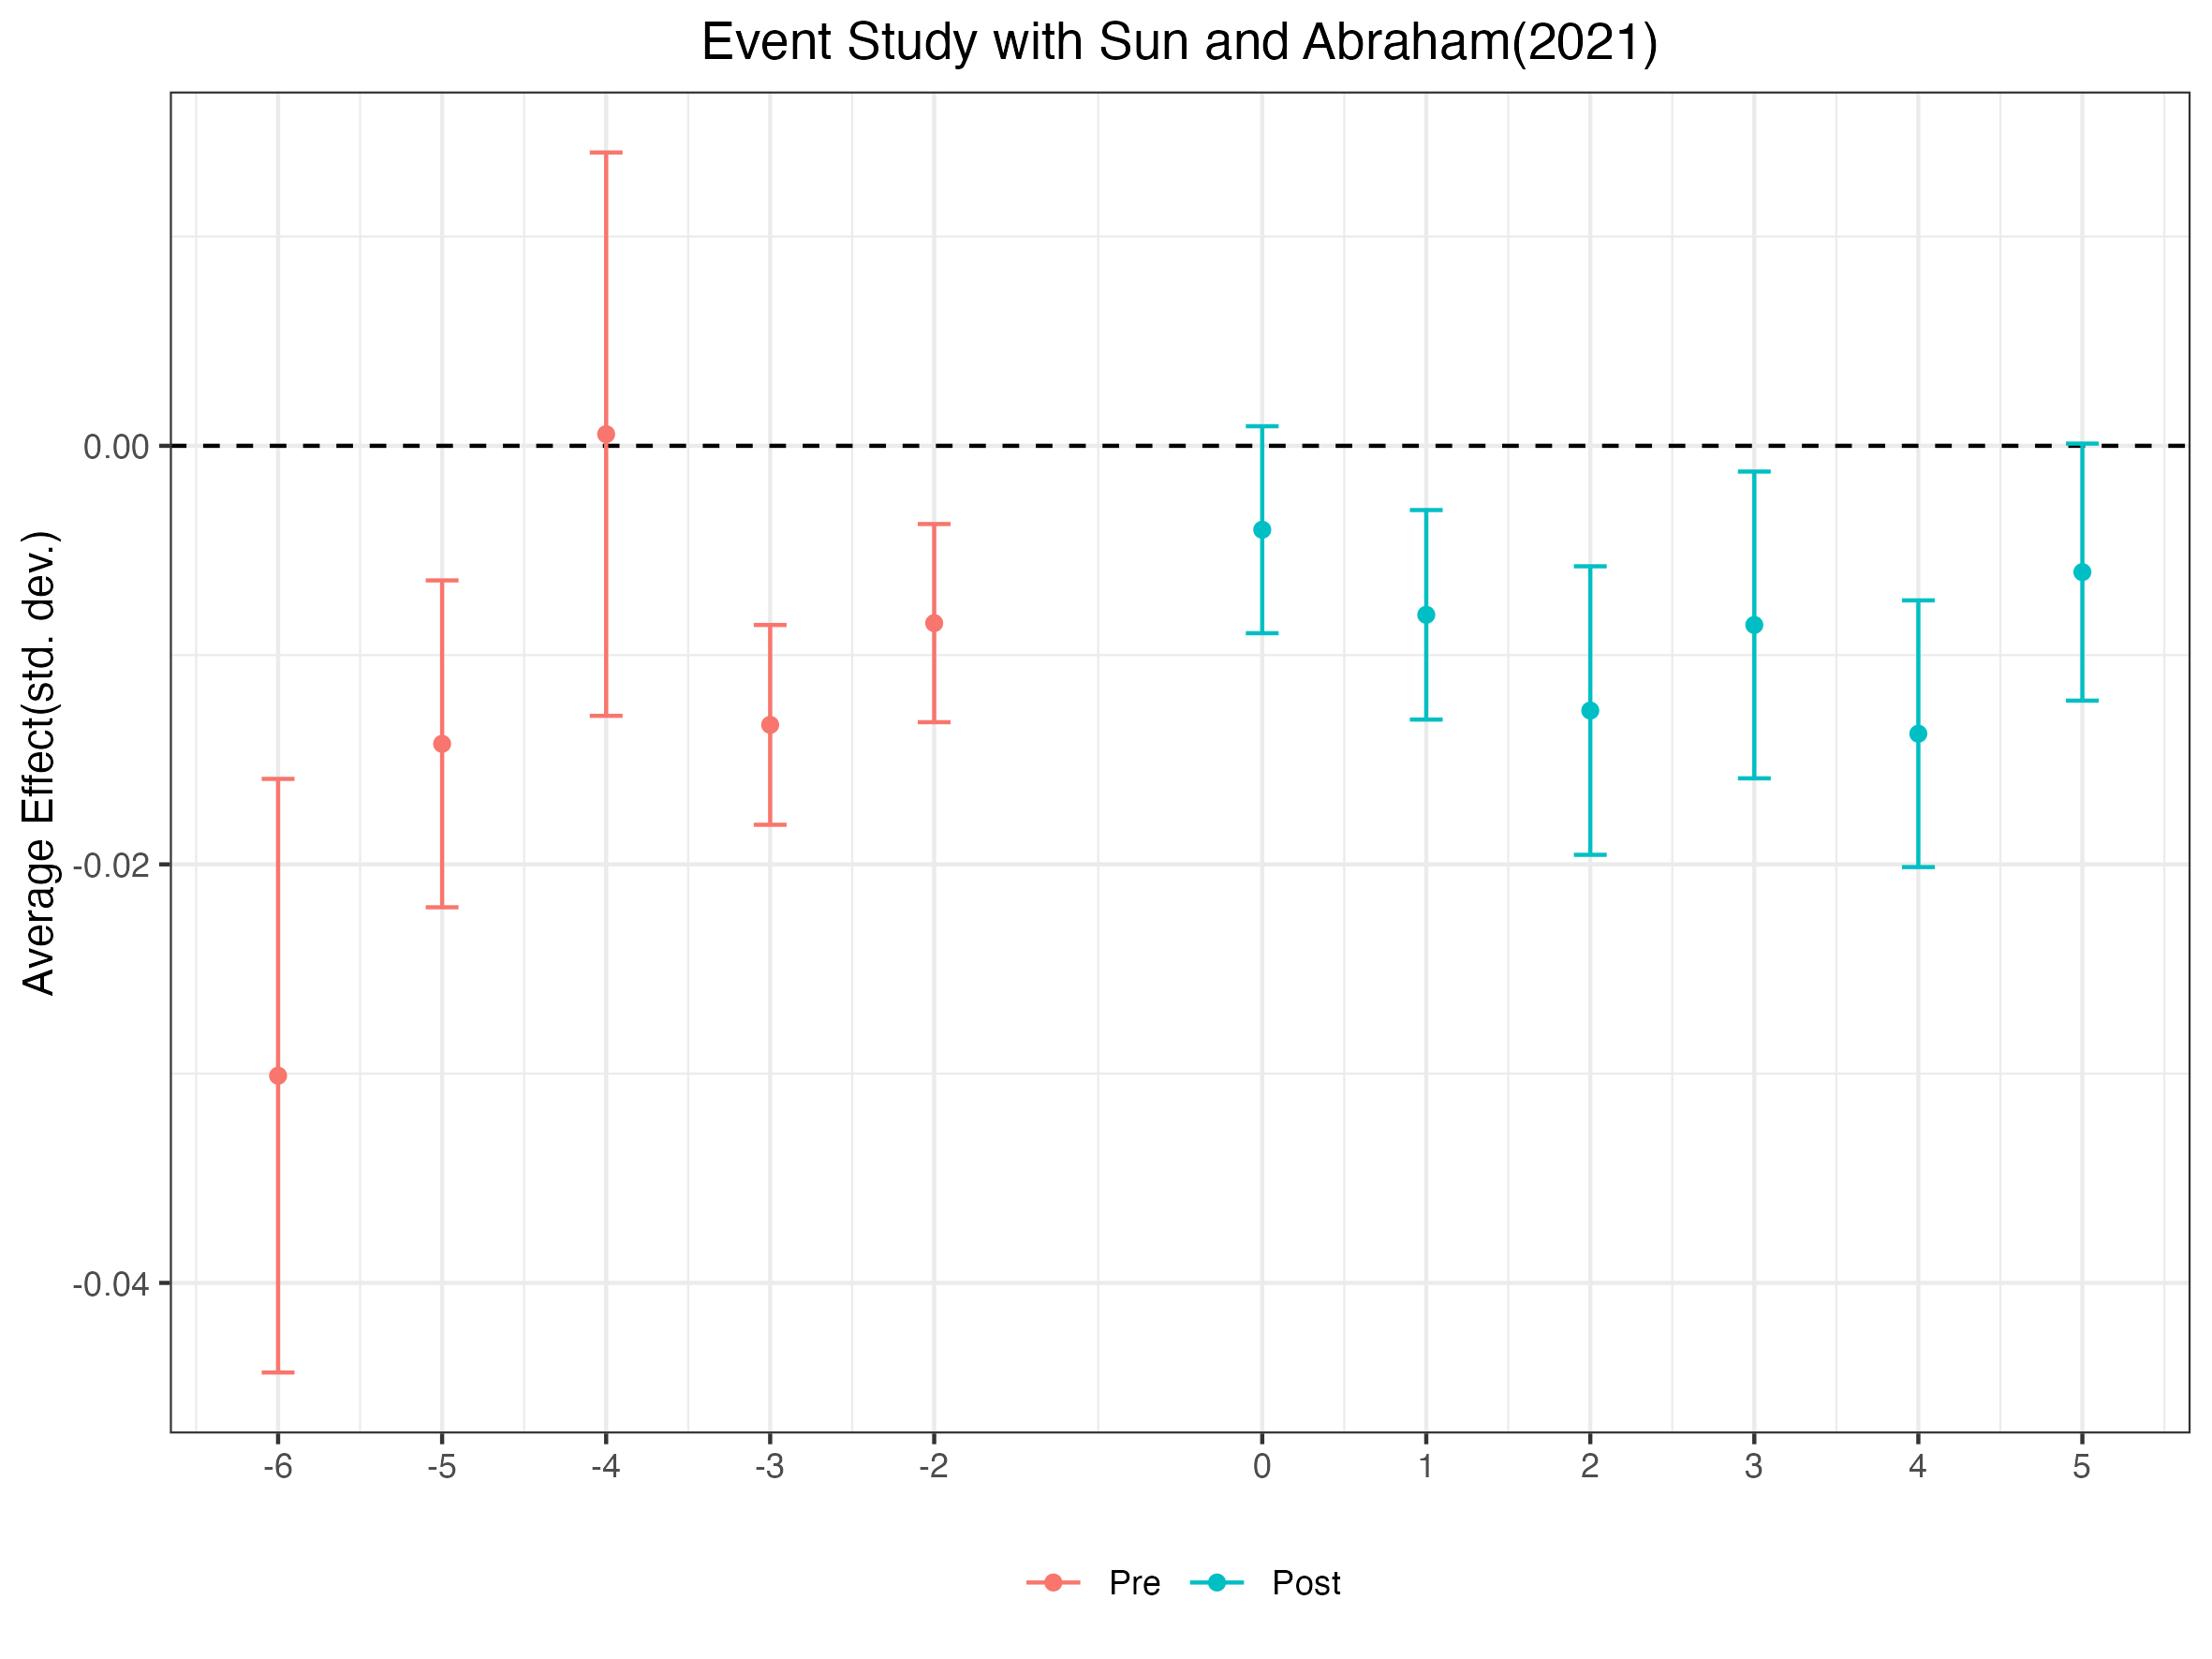
\includegraphics[width=0.7\textwidth, height=8.5cm]{figures/did-base/sadid(high school attendance).png}
    \captionsetup{width=0.7\textwidth}
    \caption{Event Study: High School Attendance}
    \label{fig:high school shares}
    \begin{minipage}{0.7\textwidth}
    \scriptsize
    Notes: The figure shows the event study results of the high school attendance among individuals between age 16 and 18 (inclusive) based on SA-DiD. 
    The base period is set to the year before the shale boom started in each state.
    The point estimates can be interpreted as the percentage point change in college enrollment status with respect to the treatment (i.e., the shale boom).
    Standard errors are clustered at the state level and the confidence intervals shown are 95\% confidence intervals.
    \end{minipage}
\end{figure}

\begin{figure}[htbp]
    \centering
    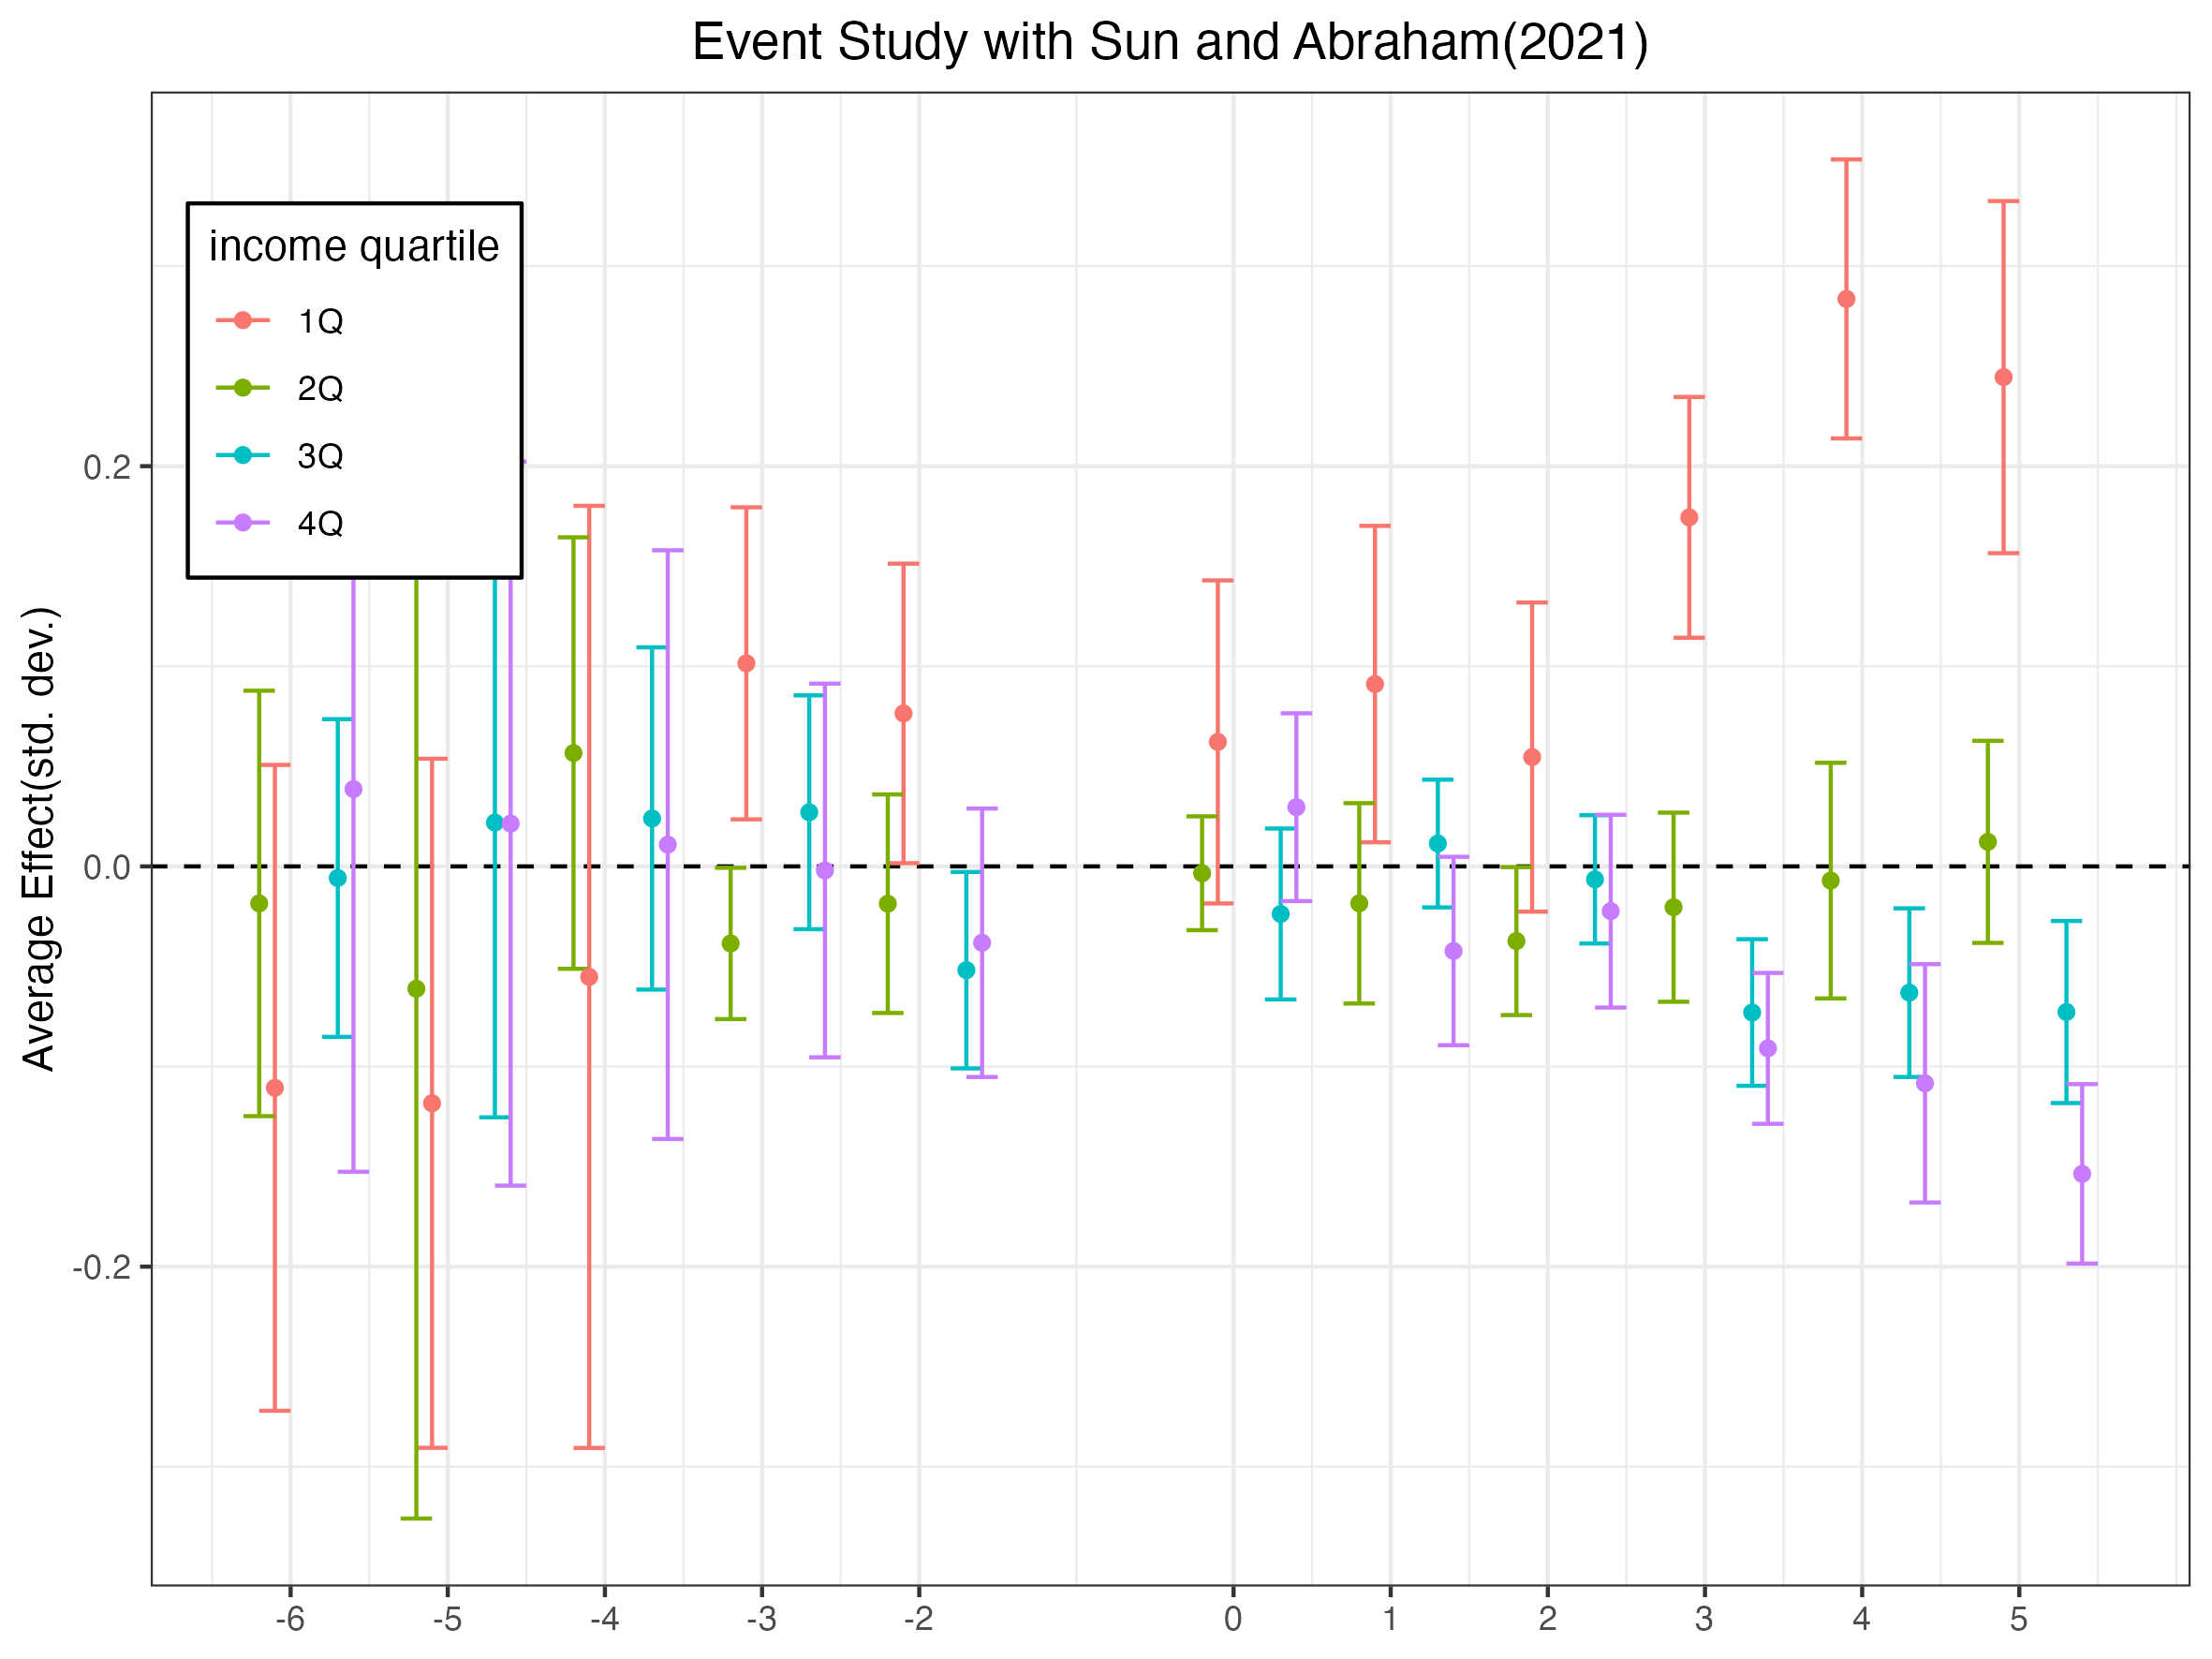
\includegraphics[width=0.7\textwidth]{figures/did-base/sadid(high school attendance- by income quartile).png}
     \captionsetup{width=0.7\textwidth}
    \caption{Event Study: High School Attendance by Household Income Quartile}
    \label{fig:high school shares - by quartile}
    \begin{minipage}{0.7\textwidth}
    \scriptsize
    Notes: The figure shows the event study results of the high school attendance among individuals between age 16 and 18 (inclusive) by family income quartile based on SA-DiD. 
    The base period is set to the year before the shale boom started in each state.
    The point estimates can be interpreted as the percentage point change in college enrollment status with respect to the treatment (i.e., the shale boom).
    Standard errors are clustered at the state level and the confidence intervals shown are 95\% confidence intervals.
    Also, note that the cutoffs for income quartiles are nation-level quartiles adjusted by the sampling weights and is fluctuant across years.
    \end{minipage}
\end{figure}


\begin{figure}[htbp]
    \centering
    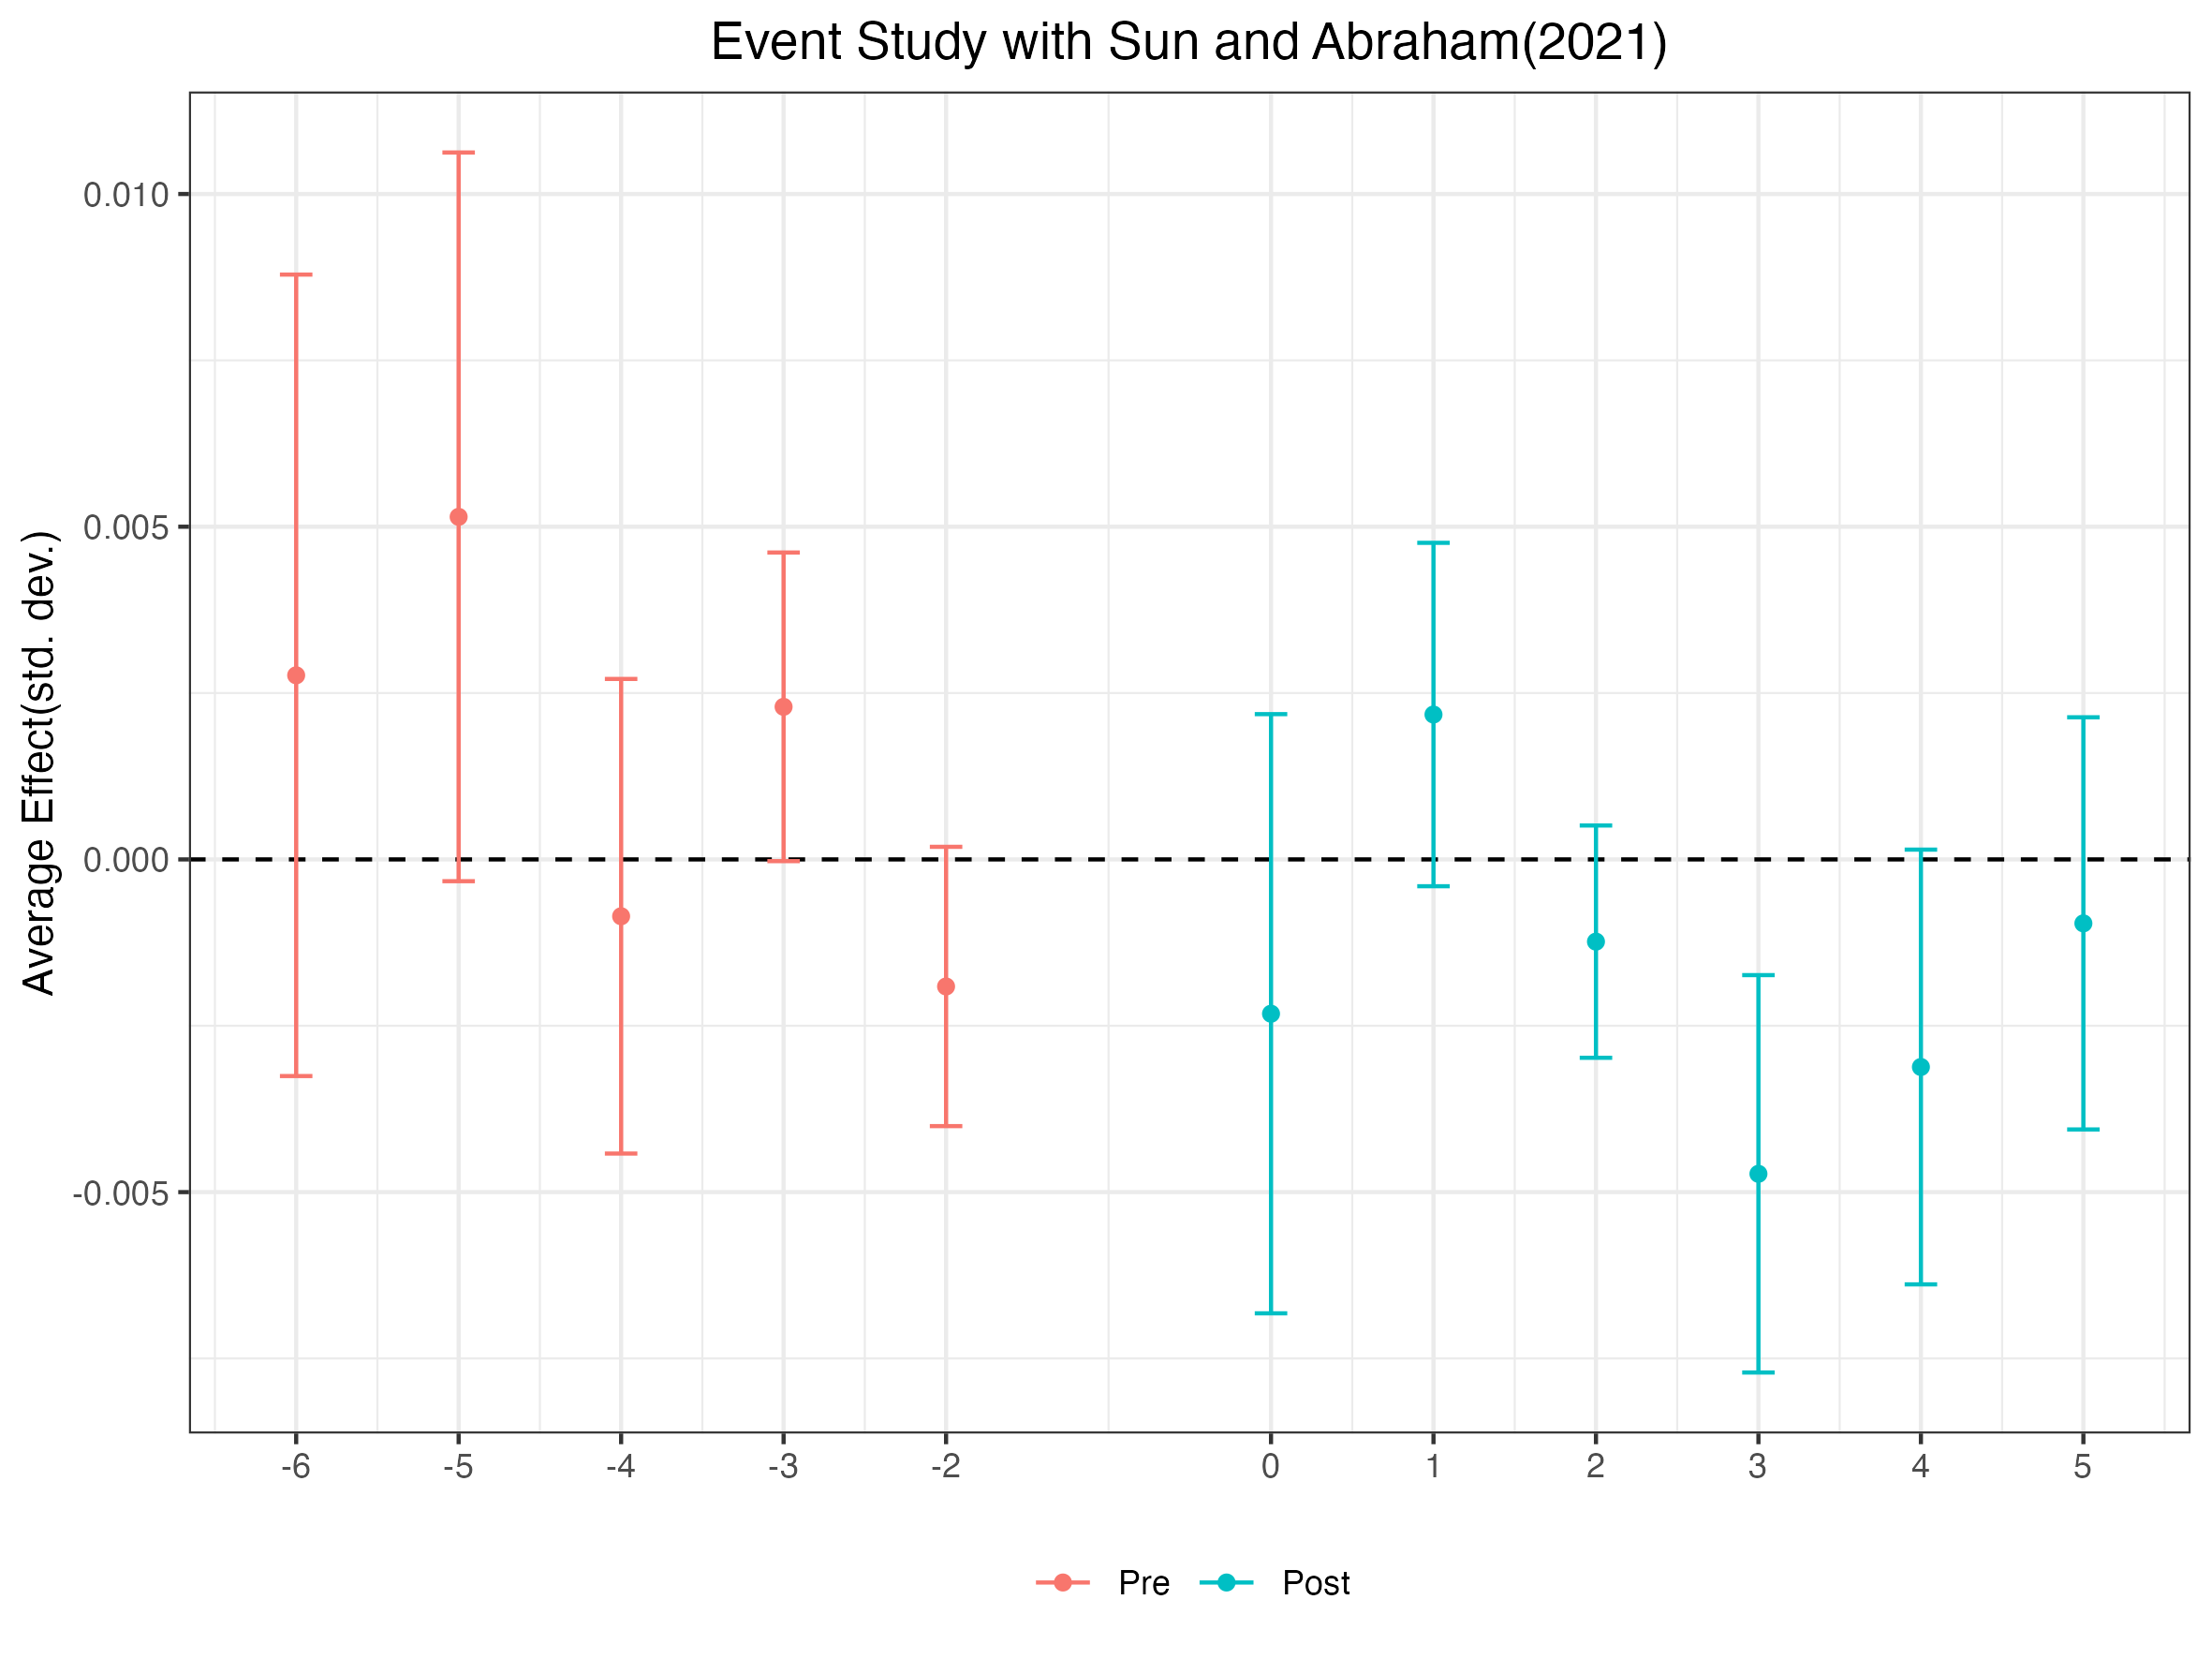
\includegraphics[width=0.7\textwidth, height=8.5cm]{figures/did-base/sadid(young school attendance).png}
     \captionsetup{width=0.7\textwidth}
    \caption{Event Study: Elementary School Attendance}
    \label{fig:elementary school shares}
    \begin{minipage}{0.7\textwidth}
    \scriptsize
     Notes: The figure shows the event study results of the elementary school attendance among individuals between age 5 and 10 (inclusive) based on SA-DiD. 
    The base period is set to the year before the shale boom started in each state.
    The point estimates can be interpreted as the percentage point change in college enrollment status with respect to the treatment (i.e., the shale boom).
    Standard errors are clustered at the state level and the confidence intervals shown are 95\% confidence intervals.
    \end{minipage}
\end{figure}

\begin{figure}[htbp]
    \centering
    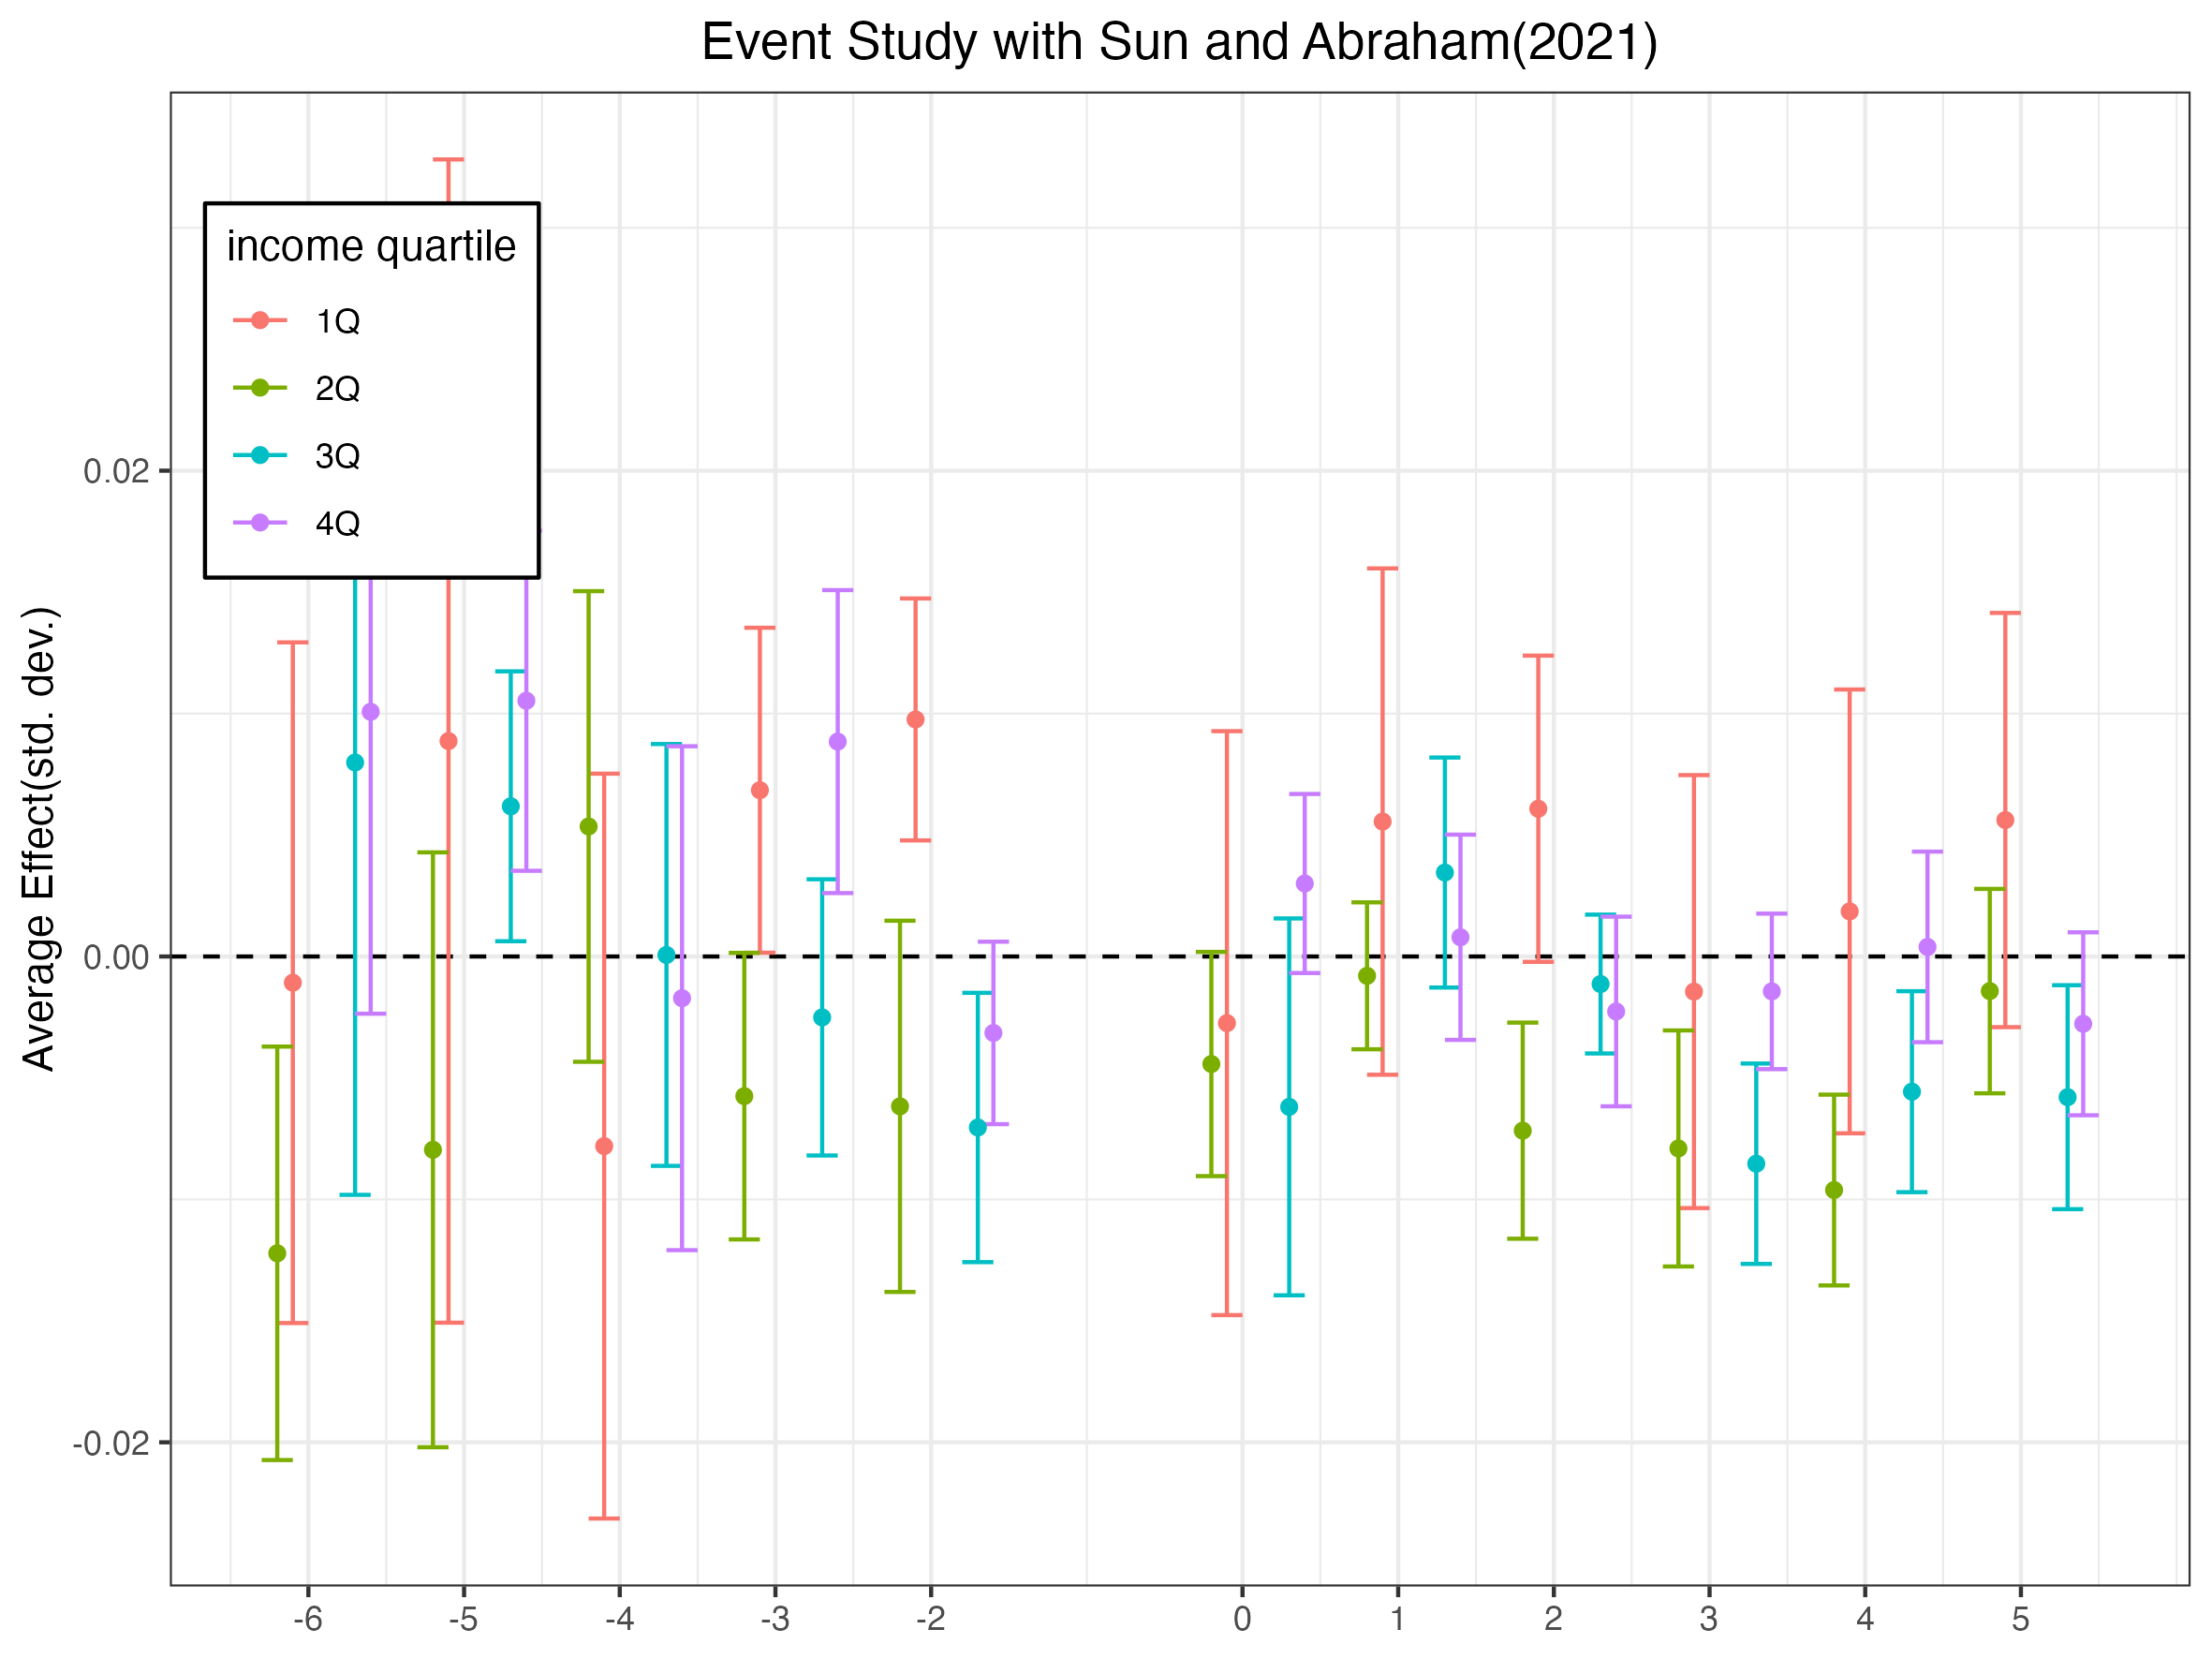
\includegraphics[width=0.7\textwidth]{figures/did-base/sadid(young school attendance - by income quartile).png}
     \captionsetup{width=0.7\textwidth}
    \caption{Event Study: Elementary School Attendance by Household Income Quartile}
    \label{fig:elementary school shares - by quartile}
    \begin{minipage}{0.7\textwidth}
    \scriptsize
    Notes: The figure shows the event study results of the elementary school attendance among individuals between age 5 and 10 (inclusive) by family income quartile based on SA-DiD. 
    The base period is set to the year before the shale boom started in each state.
    The point estimates can be interpreted as the percentage point change in college enrollment status with respect to the treatment (i.e., the shale boom).
    Standard errors are clustered at the state level and the confidence intervals shown are 95\% confidence intervals.
    Also, note that the cutoffs for income quartiles are nation-level quartiles adjusted by the sampling weights and is fluctuant across years.
    \end{minipage}
\end{figure}


\begin{figure}[htbp]
    \centering
    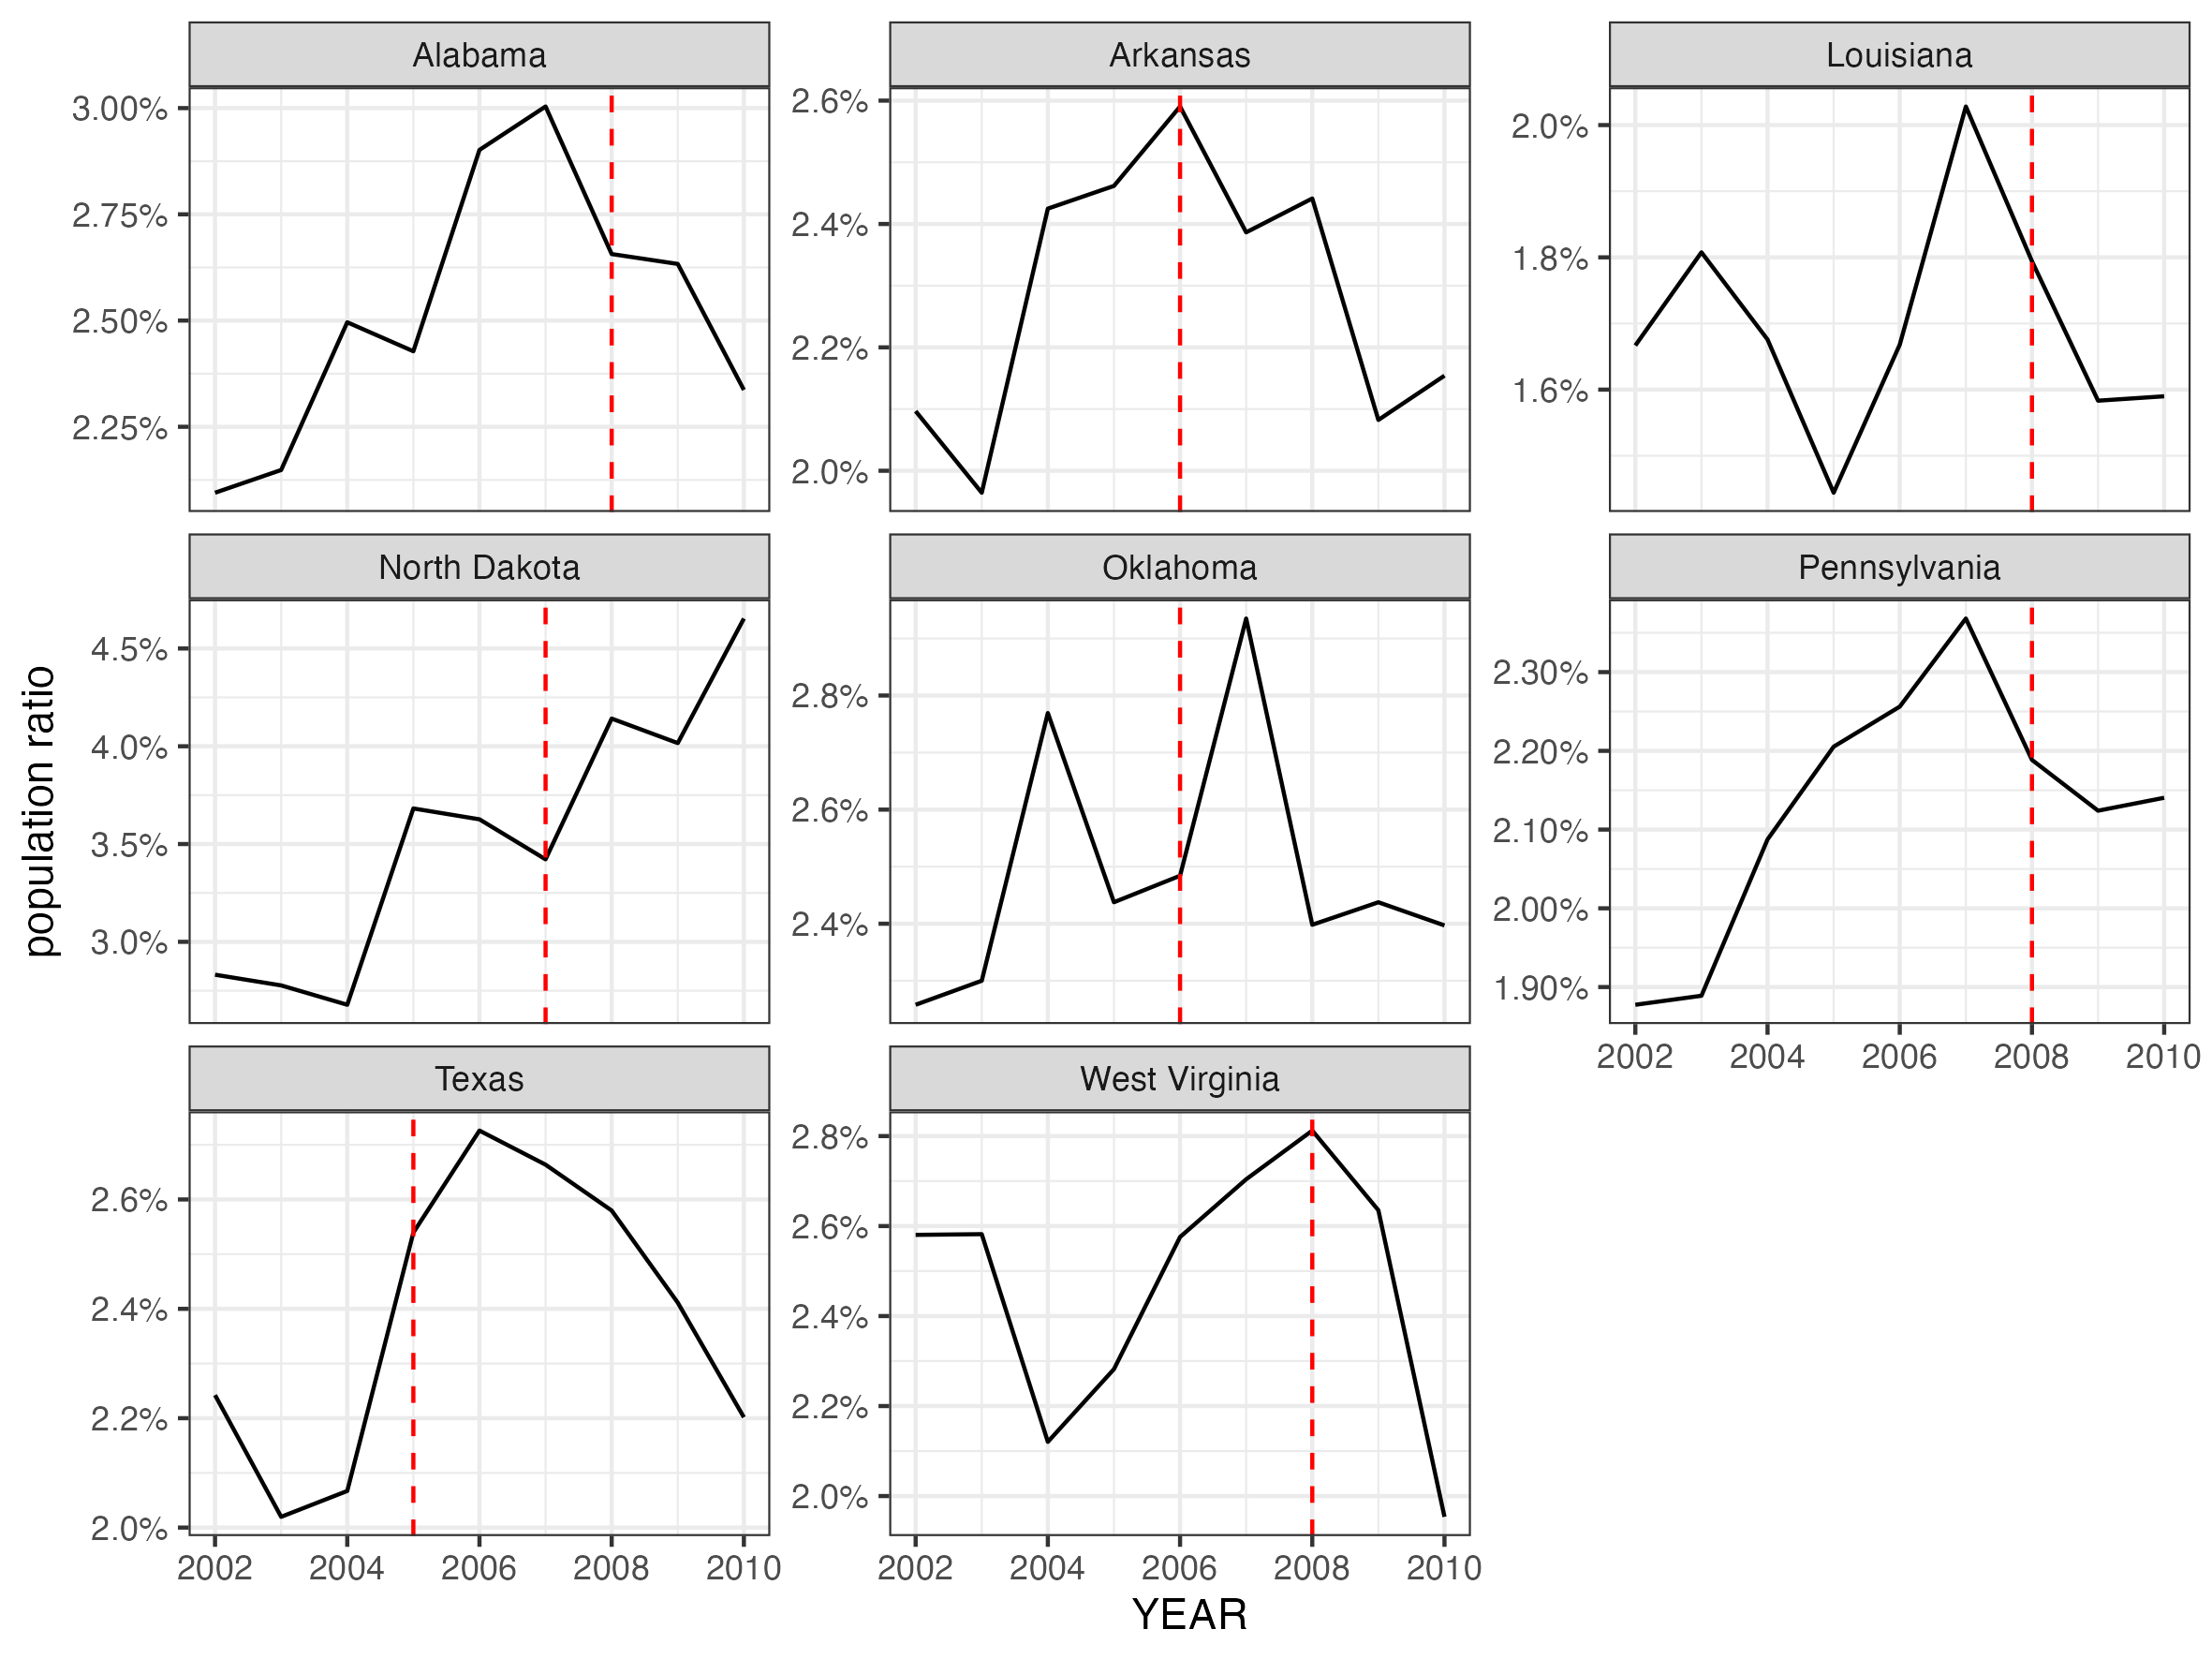
\includegraphics[width=0.7\textwidth]{figures/pop_ratio_from_outside.png}
    \captionsetup{width=0.7\textwidth}
    \caption{Population Ratio of Migrants from Outside Shale States}
    \label{fig:migration_share}
    \begin{minipage}{0.7\textwidth}
    \scriptsize
    Notes: The figure displays the population ratio of individuals who
    moved from outside the shale states to inside the shale states within a year.
    The population ratio is calculated as the (weighted) number of individuals who moved from outside the shale states to inside the shale states divided by the total population of the shale states.
    \end{minipage}
\end{figure}

\begin{figure}[htbp]
    \centering
    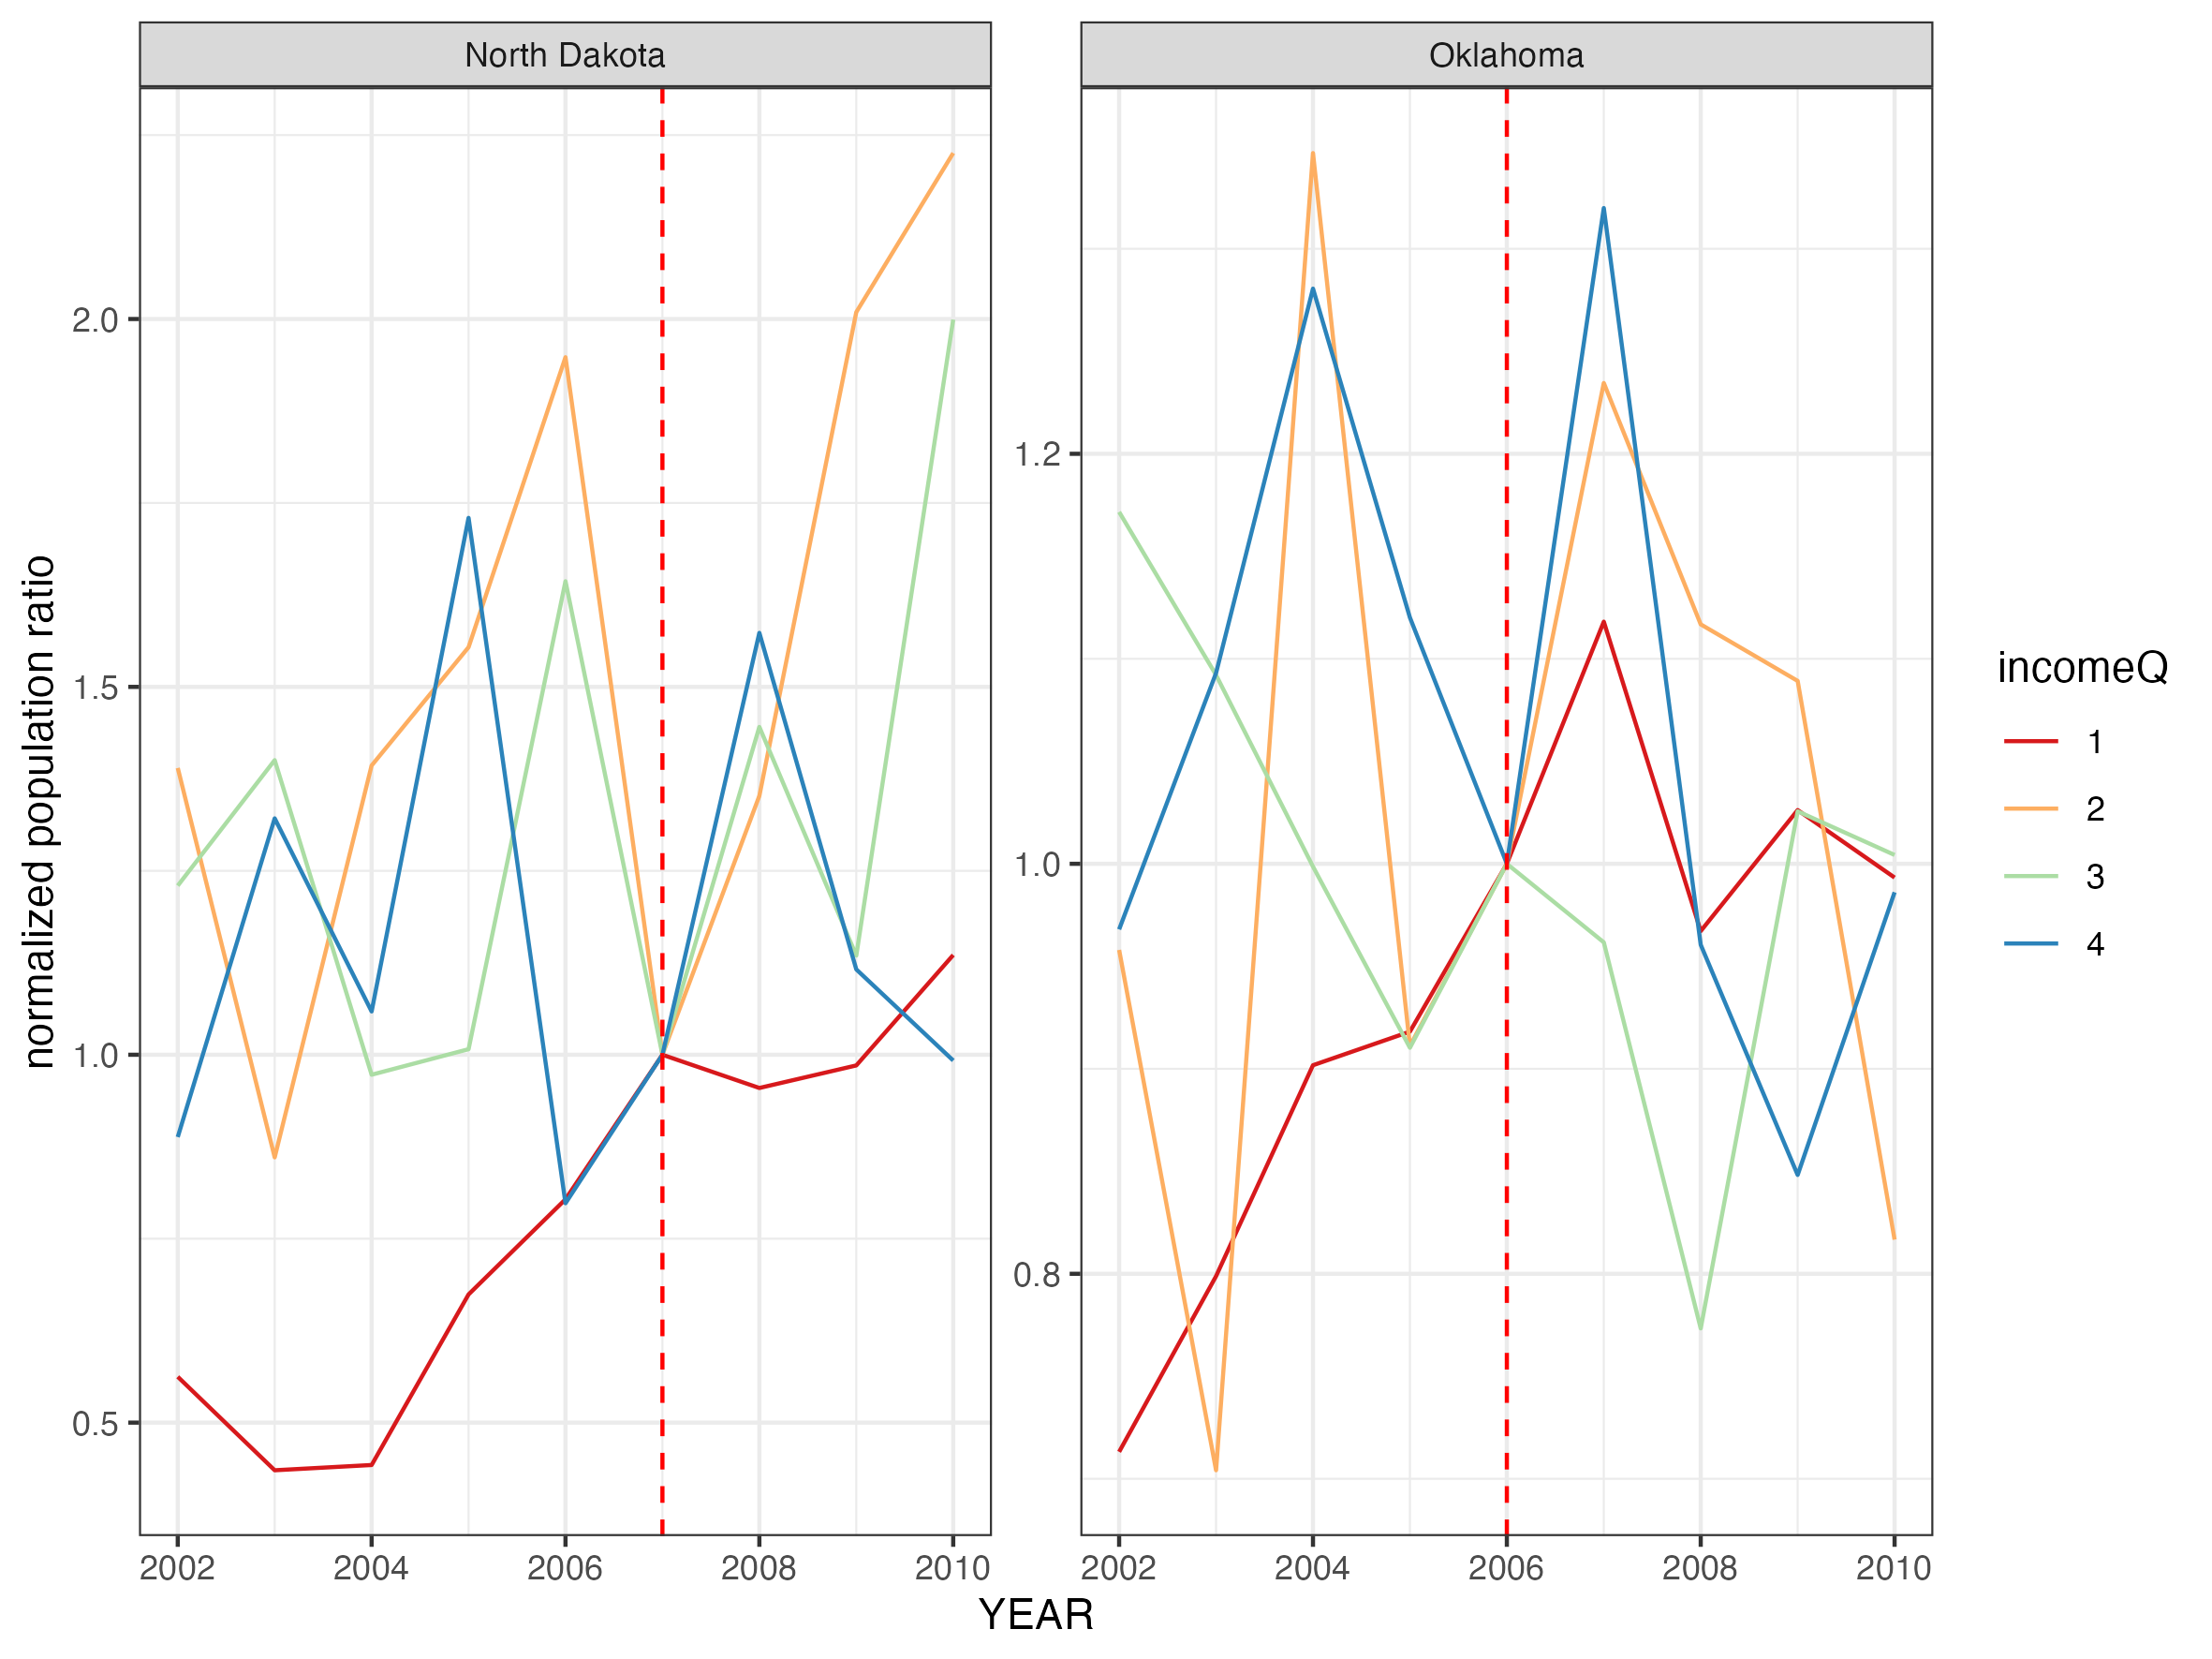
\includegraphics[width=0.7\textwidth]{figures/pop_ratio_from_outside - by income quartile.png}
    \captionsetup{width=0.7\textwidth}
    \caption{Normalized Population Ratio of Migrants from Outside Shale State by Personal Income Quartile(North Dakota and Oklahoma)}
    \label{fig:migration_share-by quartile}
    \begin{minipage}{0.7\textwidth}
    \scriptsize
    Notes: The figure displays the normalized population ratio of individuals who
    moved from outside the shale states to inside the shale states within a year.
    The normalization is done by dividing the population ratio of each income quartile group by the population ratio in the 
    year of shale boom start in each state (e.g., 2005 for Texas) – which helps focus on the relative changes in the population ratio of each income quartile group.
    Note that these income quartiles are based on personal income, not household income, and are adjusted by the sampling weights.
    The raw population ratio before normalization is calculated as the (weighted) number of individuals who moved from outside the shale states to inside the shale states divided by the total population of the shale states.
    \end{minipage}
\end{figure}
